\chapter{Black hole formation 2: Vaidya collapse}
\label{s:vai}

\minitoc

\section{Introduction}

Having investigated the gravitational collapse of a star, modelled as a ball of dust,
in the preceding chapter, we move to a much less astrophysical scenario: the
formation of a black hole by the collapse of a spherical shell of pure radiation
(no matter!).
Albeit quite academic, this process illustrates various features of black hole birth and dynamics,
in a way somewhat complementary to the collapse of a ball of dust.
The model is based on an exact solution of the Einstein equation sourced by
a pure radial electromagnetic flux, known as \emph{Vaidya metric}, which
we present first (Sec.~\ref{s:vai:Vaidya_metric}).
Then, we introduce the
model describing the implosion of a radiation shell and
study the black hole formation via such a process (Sec.~\ref{s:vai:infall}).
Finally, we focus on
some subclass of models giving birth a \emph{naked singularity}, i.e.
such that the central curvature is visible to remote observers located
outside the black hole region (Sec.~\ref{s:vai:naked_sing}).


\section{The ingoing Vaidya metric} \label{s:vai:Vaidya_metric}

\subsection{General expression} \label{s:vai:general}

Let us consider a spherically symmetric spacetime $(\M,\w{g})$ described by
coordinates $(v,r,\th,\ph)$ such that $v\in \R$, $r\in(0, +\infty)$,
$\th\in(0,\pi)$ and $\ph\in(0,2\pi)$, $(\th,\ph)$ being standard
spherical coordinates on $\SS^2$ and $r$ being the areal radius associated
with spherical symmetry (cf. Sec.~\ref{s:sch:static_spher}).
The \defin{ingoing Vaidya metric}\index{ingoing!Vaidya metric}\index{Vaidya!metric!ingoing --}
is the metric tensor
\be \label{e:vai:Vaidya_metric_null}
    \encadre{ \w{g} =
            -\left( 1 - \frac{2 M(v)}{r} \right)\, \dd v^2
            + 2 \, \dd v \, \dd r
        + r^2 \left( \dd\th^2 + \sin^2\th\, \dd\ph^2 \right) } ,
\ee
where $M(v)$ is a real-valued function of $v$.
We immediately notice that this expression strongly resembles that
of the Schwarzschild metric expressed in the
\emph{null ingoing Eddington-Finkelstein}\index{Eddington-Finkelstein!coordinates}\index{null!ingoing Eddington-Finkelstein coordinates}
coordinates, as given by Eq.~(\ref{e:sch:Schwarz_metric_NIEF}). Actually, the
only difference is the constant $m$ in Eq.~(\ref{e:sch:Schwarz_metric_NIEF})
replaced by the function $M(v)$ in Eq.~(\ref{e:vai:Vaidya_metric_null}).
We may even say that the Schwarzschild metric is the special case $M(v) = m$ of
the ingoing Vaidya metric.

A key property of the ingoing Vaidya metric is
\begin{greybox}
The hypersurfaces $v = \mathrm{const}$ are null; a normal to them is the (null)
vector\footnote{in index notation: $k^\alpha := - g^{\alpha\mu} \partial_\mu v = - \nabla^\alpha v \iff
k_\alpha := - \partial_\alpha v $.}:
\be \label{e:vai:def_k}
    \w{k} := - \vp{\dd v} = - \vw{\nabla} v \quad\iff\quad
    \uu{k} := - \dd v .
\ee
Moreover, $\w{k}$ is equal to minus the vector $\wpar_r$ of coordinates
$(v,r,\th,\ph)$:
\be \label{e:vai:k_d_dr}
    \w{k} = - \left. \der{}{r} \right| _{v,\th,\ph} ,
\ee
where we have rewritten $\wpar_r$ as $\left. \dert{}{r} \right| _{v,\th,\ph}$
to distinguish it from the vector $\wpar_r$ of the IEF coordinates, to be
introduced in Sec.~\ref{s:vai:IEF}.
\end{greybox}
\begin{proof}
Let $\Sigma_v$ be a hypersurface defined by $v = \mathrm{const}$.
The metric induced by $\w{g}$ on $\Sigma_v$
is obtained by setting $\dd v = 0$ in Eq.~(\ref{e:vai:Vaidya_metric_null}):
$\left.\w{g}\right| _{\Sigma_v} = r^2 \left( \dd\th^2 + \sin^2\th\, \dd\ph^2 \right)$.
This metric has clearly the signature $(0, +, +)$, i.e. it is degenerate, hence
$\Sigma_v$ is a null hypersurface (cf. Sec.~\ref{s:def:hor_as_null}).
By construction, $\w{k}$ is normal to $\Sigma_v$. It is thus a null vector.
Besides, the metric dual of
the coordinate vector field $\wpar_r$ is the 1-form
$\uu{\wpar_r} = g_{\mu r}\dd x^\mu = g_{vr} \dd v = \dd v = - \uu{k}$,
which proves Eq.~(\ref{e:vai:k_d_dr}).
\end{proof}

\begin{greybox}
Since $\dd v$ is nowhere vanishing, $\w{k}$ is a nonzero null vector field on $\M$.
We may use it to set up the \emph{time orientation} of $(\M,\w{g})$
by declaring that $\w{k}$ is future-oriented (cf. Sec.~\ref{s:fra:time_orientation}).
\end{greybox}

As shown in the notebook~\ref{s:sam:Vaidya},
the Ricci tensor of $\w{g}$ takes a simple form:
\be \label{e:vai:Ricci_tensor}
    \w{R} = \frac{2 M'(v)}{r^2}\, \dd v \otimes \dd v ,
\ee
where $M'(v)$ stands for the derivative of the function $M(v)$.
The Ricci scalar $R = g^{\mu\nu} R_{\mu\nu} = (2M'(v)/r^2) \, \nabla_\mu v \nabla^\mu v =  (2M'(v)/r^2) \, k_\mu k^\mu$ is identically zero, since $\w{k}$ is a null vector.
It follows that
\begin{greybox}
The ingoing Vaidya metric (\ref{e:vai:Vaidya_metric_null}) is a solution
of the Einstein equation (\ref{e:fra:Einstein_eq})
with $\Lambda = 0$ and with the energy-momentum tensor
\be \label{e:vai:ener_mom_tensor}
   \encadre{ \w{T} = \frac{M'(v)}{4\pi r^2}\, \uu{k} \otimes \uu{k}  } .
\ee
\end{greybox}

\begin{remark}
We have already noticed that Vaidya metric reduces to Schwarzschild metric for $M(v) = \mathrm{const}$.
This corresponds to $M'(v) = 0$, so that
Equation~(\ref{e:vai:ener_mom_tensor}) reduces to $\w{T} = 0$ and we recover that
Schwarzschild metric is a solution of the vacuum Einstein equation.
\end{remark}

The tensor (\ref{e:vai:ener_mom_tensor}) has the same
structure as the energy-momentum tensor of the dust model considered in Chap.~\ref{s:lem}:
$\w{T}_{\rm dust} = \rho  \, \uu{u} \otimes \uu{u} $ [Eq.~(\ref{e:lem:T_pressureless})].
The main difference is that $\w{u}$ is a timelike vector (the dust 4-velocity), while
$\w{k}$ is a null vector. For this reason, the energy-momentum tensor  (\ref{e:vai:ener_mom_tensor})
is sometimes referred to as a \defin{null dust}\index{null!dust}\index{dust!null --} model \cite{Poiss04}.
It corresponds physically to the energy-momentum tensor of some \emph{monochromatic electromagnetic radiation} in the
\emph{geometrical optics}\index{geometrical optics} approximation (see Box~22.4 of Ref.~\cite{MisneTW73}):
$\w{T}_{\rm rad} = q  \, \uu{K} \otimes \uu{K}$, where $q\geq 0$ and $\w{K} := \vw{\nabla}\Phi$ is the \emph{wave vector}\index{wave!vector}, $\Phi$ being the rapidly-varying
phase in the geometrical optics decomposition $\w{A} = \mathrm{Re}(\mathrm{e}^{\mathrm{i}\Phi} \, \w{a})$ of the electromagnetic potential 1-form $\w{A}$. The quantity $q$ is related to the energy density
$\veps$ of the electromagnetic field as measured by an observer $\Obs$ of 4-velocity $\w{u}$
by $\veps = \omega^2 q$, where $\omega = - \w{K}\cdot\w{u}$ is the frequency of the electromagnetic
radiation as measured by $\Obs$.
Maxwell equations\index{Maxwell equations} imply that $\w{K}$ is a null vector and that it is geodesic:
$\w{\nabla}_{\w{K}}\, \w{K} = 0$. The geodesic integral curves of $\w{K}$ are nothing but
the \emph{light rays}\index{light!ray} of the geometrical optics framework.
The geodesic character also holds for $\w{k}$ as defined by Eq.~(\ref{e:vai:def_k}),
since $\w{k}$ is normal to the null hypersurfaces $v = \mathrm{const}$:
the integral curves of $\w{k}$ are the null geodesic generators of these hypersurfaces
(cf. Sec.~\ref{s:def:null_geod_gen}); moreover,
we have exactly
\be \label{e:vai:k_geodesic}
    \w{\nabla}_{\w{k}}\, \w{k} = 0 .
\ee
This follows from Eq.~(\ref{e:def:wl_geod_kappa}) with $\wl = \w{k}$ and $\kappa = 0$
by virtue of Eq.~(\ref{e:def:def_kappa}) with $\rho=0$ implied by
Eq.~(\ref{e:def:wl_rho_u}) given that $u = v$ and $\w{k} =  - \vw{\nabla} v$ [Eq.~(\ref{e:vai:def_k})].
Equations~(\ref{e:vai:k_geodesic}) and (\ref{e:vai:k_d_dr})
imply that the curves $(v,\th,\ph) = \mathrm{const}$
are null geodesics, $\lambda:=-r$ is an affine parameter along them and $\w{k}$ is
the corresponding tangent vector.

Another condition for the identification of $\w{T}$ with $\w{T}_{\rm rad}$ is that the coefficient
in front of $\uu{k} \otimes \uu{k}$ in (\ref{e:vai:ener_mom_tensor})
is non-negative, since $q\geq 0$ in $\w{T}_{\rm rad}$. This constraint can also be seen as the \emph{null energy condition} (\ref{e:neh:null_energy_cond}) introduced in
Sec.~\ref{s:neh:NEH_Theta_zero}: for any null vector $\wl$, we have
$\w{T}(\wl,\wl) = M'(v)/(4\pi r^2)\, (\w{k}\cdot\wl)^2$ and hence $\w{T}(\wl,\wl) \geq 0$ $\iff$
$M'(v) \geq 0$. In other words, the function $M(v)$ must be monotically increasing. Then, we can set
$\w{k} = \alpha \w{K}$, where $\alpha$ is a constant, to have a perfect match of (\ref{e:vai:ener_mom_tensor}) with the electromagnetic radiation energy-momentum
tensor $\w{T}_{\rm rad}$.
To summarize:
\begin{greybox}
Provided that $M(v)$ is an increasing function\footnote{by \emph{increasing}, it is meant
strictly increasing ($M'(v)>0$) or locally constant ($M'(v) = 0$).},
the ingoing Vaidya spacetime $(\M,\w{g})$ is generated by a spherical symmetric electromagnetic radiation
within the geometrical optics approximation. The corresponding light rays are the
\defin{ingoing radial null geodesics}\index{ingoing!radial!null geodesics}
$\Li^{\rm in}_{(v,\th,\ph)}$
defined by $v=\mathrm{const}$, $\th=\mathrm{const}$ and $\ph=\mathrm{const}$.
These geodesics admit $\w{k}$ as the tangent vector associated with their affine parameter
$\lambda := -r$.
\end{greybox}

\begin{hist} \label{h:vai:origin}
Vaidya metric has actually been first derived by Henri Mineur\index{Mineur, H.} in 1933 \cite{Mineu1933},
as the solution of the Einstein equation for the exterior of a spherically symmetric body,
the ``mass'' of which ``is varying''
due to the radiation of a ``energy flux of light''. It thus corresponds to the \emph{outgoing}
version of Vaidya metric, while the version (\ref{e:vai:Vaidya_metric_null})
considered here is \emph{ingoing}. More precisely, the solution given by Mineur
reads\footnote{This is Mineur's Eq.~(21), p.~47 of Ref.~\cite{Mineu1933}.
The minus sign in the left-hand side, which is present
Mineur's article~\cite{Mineu1933}, is fortunate for comparison with the current text
since Mineur is using the metric signature $(+,-,-,-)$, i.e. the opposite of ours.}
\be \label{e:vai:Mineur_metric}
   -\D s^2 = 2 \,  \D x \,  \D r + r^2 \, \frac{\D u^2 - \D v^2}{u^2} - \left( 1 - \frac{2 M(x)}{r} \right) \D x^2 .
\ee
The coordinate $x$ is the opposite of a retarded time ($x = -u$ in our notations), while $(u,v)$ are coordinates on the 2-sphere $\SS^2$ (submanifold $(x,r) = \mathrm{const}$)
such that the standard (round)
metric of $\SS^2$  is $\w{q} = u^{-2} \left( - \dd u^2 + \dd v^2 \right)$
(cf. the unnumbered equation at the top of p.~35 of Mineur's article \cite{Mineu1933}).
This looks quite surprising, given that $u^{-2} \left( - \dd u^2 + \dd v^2 \right)$
is rather the metric of the 2-dimensional anti-de Sitter space expressed in a variant
of Poincaré coordinates (compare Eq.~(\ref{e:exk:metric_AdS2}) with $T = v$ and $R = 1/u$).
In particular the signature is $(-, +)$, while it should be $(+,+)$ for
$\SS^2$! It turns out that the coordinate $u$ used by Mineur is pure imaginary,
i.e. Mineur wrote the metric of $\SS^2$ via a kind of Wick rotation of
the metric of the hyperbolic plane\index{hyperbolic!plane}\footnote{The spaces $\mathbb{H}^2$ and $\SS^2$
are somehow connected as being the only 2-dimensional Riemannian manifolds of
nonzero constant scalar curvature (negative for $\mathbb{H}^2$ and positive for $\SS^2$).}
 $\mathbb{H}^2$, the latter being
$(\dd X^2 + \dd Y^2)/Y^2$: setting $v = X$ and $u = \mathrm{i} Y$, one
gets $-\w{q} =  u^{-2} \left( \dd u^2 - \dd v^2 \right)$. If one restores
the standard spherical coordinates $(\th,\ph)$ on $\SS^2$ and uses the modern notation
$u = -x$ as well as the metric signature $(-,+,+,+)$, one can rewrite Mineur's
solution as\footnote{As one can infer by comparing with other expressions
of $\D s^2$ in Mineur's article, the $+$ sign in front of $r^2$ times the $\SS^2$
line element in Eq.~(\ref{e:vai:Mineur_metric}) is certainly a typo and should be
replaced by a $-$ sign; this correction is performed to get Eq.~(\ref{e:vai:Mineur_metric_modern}).}
\be \label{e:vai:Mineur_metric_modern}
   \w{g} = -\left( 1 - \frac{2 M(u)}{r} \right)\, \dd u^2
            -  2 \, \dd u \, \dd r
        + r^2 \left( \dd\th^2 + \sin^2\th\, \dd\ph^2 \right) .
\ee
This ressembles the metric (\ref{e:vai:Vaidya_metric_null}).
The only difference is the $-$ sign in front of $\dd u \, \dd r$, while there is a $+$ sign
in front  $\dd v \, \dd r$ in (\ref{e:vai:Vaidya_metric_null}). This results form Mineur's version
being \emph{outgoing}, given that he considered a radiating body. On
the contrary, the version (\ref{e:vai:Vaidya_metric_null}) is \emph{ingoing}, since we are interested in gravitational collapse and black hole formation.

Only 20 years later, in 1953, Prahalad Chunnilal Vaidya\index{Vaidya, P.C.} did publish
the metric that bears his name in the form (\ref{e:vai:Mineur_metric_modern}) \cite{Vaidy53}.
Previously, in 1943 \cite{Vaidy43} and in 1951 \cite{Vaidy51a}, Vaidya presented
the metric outside a spherically symmetric radiating star in an equivalent, but
more complicated form:
\be \label{e:vai:Vaidya_metric_original}
    \w{g} = - \frac{1}{f(M)^2} \left( \der{M}{T} \right) ^2
    \left(1 - \frac{2 M}{r} \right) \, \dd T^2
    + \left(1 - \frac{2 M}{r} \right) ^{-1} \dd r^2
        + r^2 \left( \dd\th^2 + \sin^2\th\, \dd\ph^2 \right) ,
\ee
where $f$ is an arbitrary function and $M = M(T, r)$ fulfils the differential equation
$\dert{M}{r}\, (1 - {2 M}/{r}) = f(M)$.
By introducing the scalar field $u$ such that $\dd u = - f(M)^{-1} \dd M$
and promoting it as a coordinate, one can
bring this solution to Mineur's form (\ref{e:vai:Mineur_metric_modern}).
In a foreword to Vaidya's 1951 article \cite{Vaidy51a},
Vishnu Vasudev Narlikar\index{Narlikar, V.V.}, who was Vaidya's PhD advisor,
wrote: \emph{``The treatment as given here is essentially different from that of Professor H. Mineur
as it appears in Ann. de l'Ecole Normal Superieure, Ser. 3, 5, 1, 1933
\emph{(our Ref. \cite{Mineu1933})}. Our attention
was kindly drawn to it by Professor Mineur some years ago.''} In a common article by
Narlikar and Vaidya published in 1947 \cite{NarliV1947}, one can also read
\emph{``The line element (5) \emph{[our Eq.~(\ref{e:vai:Vaidya_metric_original})]}
was first published by one of us some years ago. A line element equivalent to
(5) but not obviously so was obtained by Mineur
several years earlier.''} It would probably be fair to call the metric
(\ref{e:vai:Mineur_metric_modern}) the \emph{Mineur-Vaidya metric}; however,
we keep here the usual name of \emph{Vaidya metric}.
The metric (\ref{e:vai:Mineur_metric_modern}) was popularized and further studied by Richard W. Lindquist\index{Lindquist, R.W.}, Robert A. Schwartz\index{Schwartz, R.A} and Charles W. Misner\index{Misner, C.W.}
in 1965 \cite{LindqSM65}.
\end{hist}

\subsection{Expression in ingoing Eddington-Finkelstein coordinates} \label{s:vai:IEF}

To deal with black hole formation in Vaidya spacetime, it is quite
convenient to work with the
\defin{ingoing Eddington-Finkelstein (IEF) coordinates}\index{Eddington-Finkelstein!coordinates}\index{ingoing!Eddington-Finkelstein!coordinates}\index{IEF}
$(t,r,\th,\ph)$, which are defined from the null coordinates $(v,r,\th,\ph)$ in the
same way as in the Schwarzschild case, i.e. by considering that $v$ is the
\defin{advanced time}\index{advanced!time}\index{time!advanced --} with respect to $t$
[cf. Eq.~(\ref{e:sch:ti_v_r})]:
\be  \label{e:vai:t_v_r}
    \encadre{t := v - r} \iff \encadre{v = t + r} .
\ee
\begin{remark}
The coordinate $t$ was denoted by $\ti$ in Chap.~\ref{s:sch}, where $t$
was reserved for the Schwarzschild-Droste time coordinate.
\end{remark}
We have $\dd v = \dd t + \dd r$, from which the IEF expression of the
metric tensor is immediately deduced from Eq.~(\ref{e:vai:Vaidya_metric_null}):
\be \label{e:vai:metric_IEF}
    \encadre{
        \begin{array}{ll}
        \w{g} = &
           \displaystyle -\left( 1 - \frac{2 M(t+ r)}{r} \right)\, \dd t^2
            + \frac{4 M(t + r)}{r} \, \dd t \, \dd r
            + \left( 1 + \frac{2 M(t+r)}{r} \right)\, \dd r^2 \\[1ex]
       & + r^2 \left( \dd\th^2 + \sin^2\th\, \dd\ph^2 \right) .
       \end{array}
       }
\ee
The expression of $\w{k}$ in terms of the IEF coordinate frame
is deduced from Eq.~(\ref{e:vai:k_d_dr}) and the chain rule:
\be \label{e:vai:k_IEF}
    \w{k} = \wpar_t - \wpar_r .
\ee
\begin{remark}
The analog equation in Schwarzschild spacetime is Eq.~(\ref{e:sch:null_vector_k}).
\end{remark}

\subsection{Outgoing radial null geodesics}

Let us determine the radial null directions at each point by searching for
null vectors of the form $\wl = \wpar_t + V \wpar_r$. The condition
$\w{g}(\wl, \wl) = 0$ with the expression (\ref{e:vai:metric_IEF}) for
$\w{g}$ yields immediately a quadratic equation for $V$:
\[
    \left( 1 + \frac{2 M(t+r)}{r} \right) V^2
    + \frac{4 M(t + r)}{r}\, V +
    1 - \frac{2 M(t+ r)}{r}  = 0 .
\]
The two solutions are $V = -1$ and $V = [r - 2M(t + r)]/[r + 2M(t+r)]$.
The first solution gives back the ingoing null vector $\w{k}$ introduced in Sec.~\ref{s:vai:general}
[cf. Eq.~(\ref{e:vai:k_IEF})].
The null vector $\wl$ corresponding to the second solution is
\be
    \wl = \wpar_t + \frac{r - 2M(t + r)}{r + 2M(t+r)}\, \wpar_r .
\ee

\begin{greybox}
The integral curves of the vector fields $\w{k}$ and $\wl$ are null geodesics.
Those of $\w{k}$ are the \emph{ingoing radial null geodesics}\index{ingoing!radial!null geodesic}
$\Li^{\rm in}_{(v,\th,\ph)}$ already discussed in Sec.~\ref{s:vai:general},
while those of $\wl$ are called the \defin{outgoing radial null geodesics}\index{ingoing!null geodesic}.
\end{greybox}

\begin{proof}
A direct computation shows that $\wl$ is a pregeodesic vector field:
$\wnab_{\wl} \wl = \kappa \wl$, with $\kappa = - 4 [rM'(t+r) - M(t+r)]/[r + 2M(t+r)]^2$
(cf. the notebook~\ref{s:sam:Vaidya}). It follows that the integral curves of
$\wl$ are geodesics (cf. Sec.~\ref{s:geo:gener_param}).
\end{proof}
The differential equation governing the outgoing radial null geodesics
is obtained by demanding that $\wl$ is their tangent vector:
\be \label{e:vai:ODE_outgoing_null}
    \frac{\D r}{\D t} = \frac{r - 2M(t + r)}{r + 2M(t+r)} .
\ee
In what follows, we shall get exact solutions of this equation for $M(v)$ piecewise linear.

\begin{remark}
As in the Schwarzschild case (cf. Remark~\ref{r:sch:outgoing_ingoing}
on p.~\pageref{r:sch:outgoing_ingoing}),
the outgoing radial null geodesics are actually \emph{ingoing}, i.e. have $r$ decreasing towards the future,
as soon as $r < 2 M(t+r)$. This corresponds to the region bounded by the red curve in Fig.~\ref{f:vai:diag_S0}, to be discussed in Sec.~\ref{s:vai:trapped_surf}.
\end{remark}

%%%%%%%%%%%%%%%%%%%%%%%%%%%%%%%%%%%%%%%%%%%%%%%%%%%%%%%%%%%%%%%%%%%%%%%%%%%%%%%

\section{Imploding shell of radiation} \label{s:vai:infall}

\subsection{The imploding shell model} \label{s:vai:imploding_shell}

An \defin{imploding shell of radiation}\index{shell!imploding -- of radiation}\index{imploding!shell of radiation}
is defined by the ingoing Vaidya metric with the function $M(v)$ obeying
$M'(v) \neq 0$ only on a finite interval of $v$. By choosing properly
the origin of $v$, we may consider this interval to be $[0, v_0]$, with
the parameter $v_0>0$ governing the
thickness of the shell.
The function $M(v)$ is thus constant outside the interval $[0, v_0]$.
In order to describe the formation of a black hole, we choose
$M(v) = 0$ for $v < 0$. This corresponds to a piece of Minkowski spacetime,
since the metric (\ref{e:vai:metric_IEF})
clearly reduces to Minkowski metric (\ref{e:glo:Mink_metric_spher}) wherever $M(v)=0$.
Denoting by $m>0$ the constant value of $M(v)$ for $v > v_0$, we have then
\be \label{e:vai:mass_function}
    M(v) = \left\{ \begin{array}{ll}
     0 \quad \mbox{for} \ v < 0 \qquad & (\mbox{Minkowski region},\ \M_{\rm Min}) \\
     m \, S(v/v_0) \quad \mbox{for} \ 0 \leq v \leq v_0
        & (\mbox{radiation region},\ \M_{\rm rad}) \\
      m \quad \mbox{for} \ v > v_0 \qquad & (\mbox{Schwarzschild region},\ \M_{\rm Sch})
      \end{array} \right.
\ee
where $S: [0,1] \to [0,1],\ x \mapsto S(x)$ is an increasing function
obeying $S(0) = 0$ and $S(1) = 1$.
The region with $v>v_0$ is qualified as \emph{Schwarzschild} since for $M(v) = m = \mathrm{const}$,
the Vaidya metric reduces to Schwarzschild metric, as noticed
in Sec.~\ref{s:vai:general}.
The three regions are shown in terms of coordinates $(t, r)$ on Fig.~\ref{f:vai:diag_S0}:
$\M_{\rm rad}$ (the imploding shell) is the yellow region, $\M_{\rm Min}$ lies below it and
$\M_{\rm Sch}$ lies above it.

\begin{figure}
\centerline{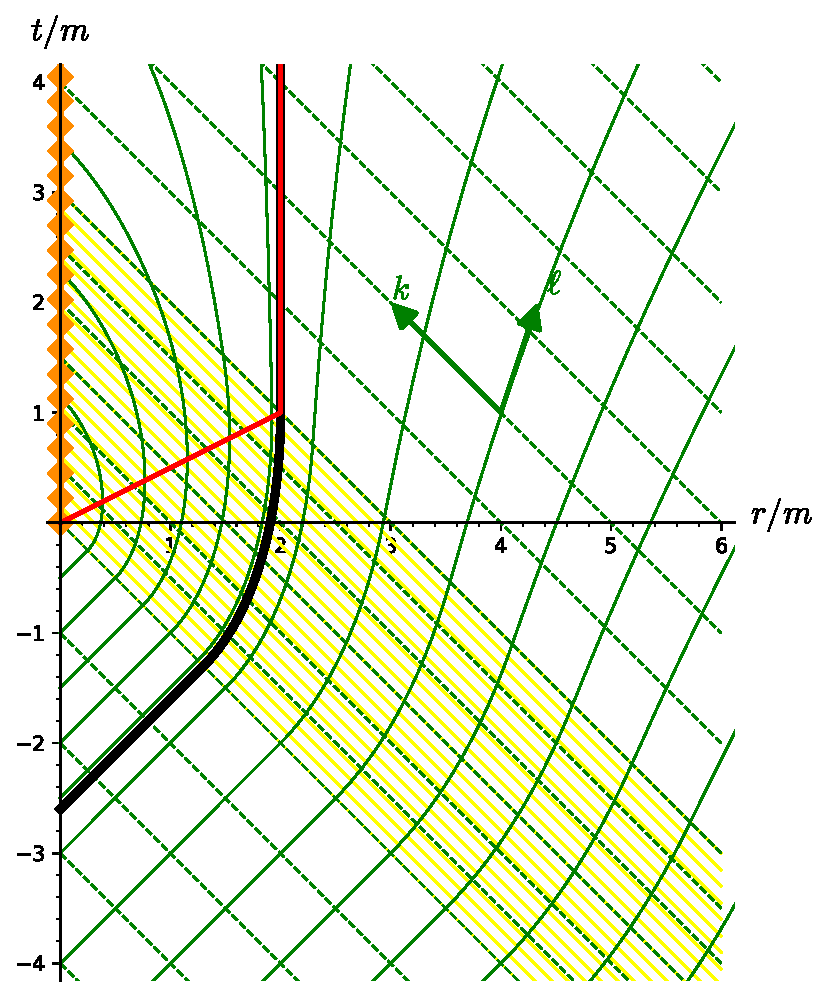
\includegraphics[width=0.6\textwidth]{vai_diag_S0.pdf}}
\caption[]{\label{f:vai:diag_S0} \footnotesize
Spacetime diagram of the Vaidya collapse based on the IEF coordinates $(t, r)$
and for the linear mass function $M(v)=m v/v_0$ with $v_0 = 3 m$
(homothetic model with $\alpha = 2/3$).
The yellow area is the radiation region $\M_{\rm rad}$
[cf. Eq.~(\ref{e:vai:mass_function})],
below it lies the Minkowski region $\M_{\rm Min}$
and above it the Schwarzschild region $\M_{\rm Sch}$.
The solid (resp. dashed) green curves are outgoing (resp. ingoing) radial
null geodesics. The thick black line marks the event horizon $\Hor$ (Sec.~\ref{s:vai:BH_formation}) and
the red one the future outer trapping horizon $\mathscr{T}$ (Sec.~\ref{s:vai:trapped_surf}).
Note that $\Hor$ and $\mathscr{T}$ coincide in $\M_{\rm Sch}$.
The curvature singularity
is indicated by the orange zigzag line. The part of the figure corresponding
to $\M_{\rm Min}$ can be compared with Fig.~\ref{f:glo:null_coord},
while that corresponding to $\M_{\rm Sch}$ can be
compared with Fig.~\ref{f:sch:rad_null_geod_EF}.
\textsl{[Figure generated by the notebook \ref{s:sam:Vaidya}]}
}
\end{figure}


The simplest example of a function $M(v)$
obeying (\ref{e:vai:mass_function}) is obtained for $S(x) = x$:
\be \label{e:vai:S_linear}
     S(x) = x \quad \iff \quad M(v) = m \frac{v}{v_0} \quad (0 \leq v \leq v_0).
\ee
It is shown as the blue curve in Fig.~\ref{f:vai:mass_function}.
This choice of $S$ makes $M(v)$ piecewise linear. The resulting metric tensor
(\ref{e:vai:Vaidya_metric_null}) is continuous but not $C^1$ at $v=0$ and $v=v_0$. A choice
of $S$ that yields a $C^2$ metric tensor is $S(x) = 6 x^5 - 15 x^4 + 10 x^3$.
This choice is depicted by the red curve in Fig.~\ref{f:vai:mass_function}.

\begin{figure}
\centerline{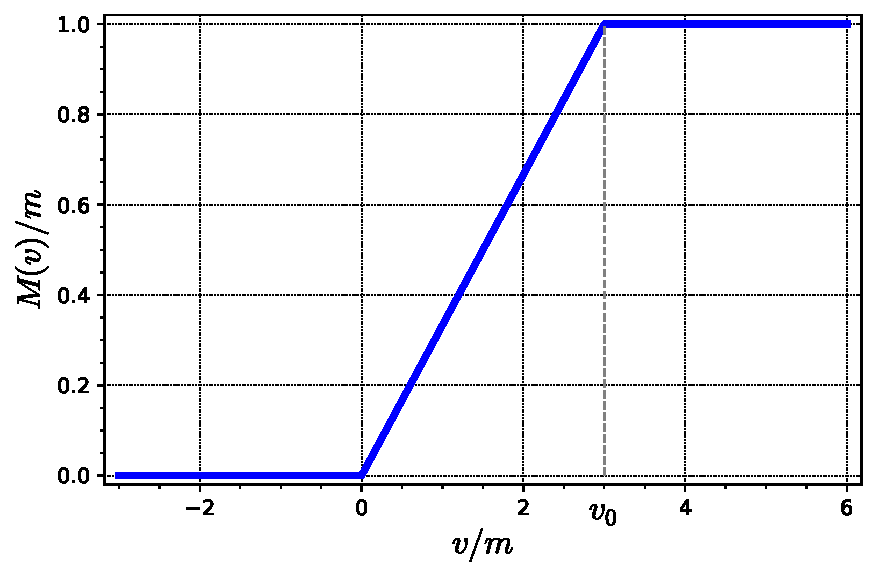
\includegraphics[width=0.6\textwidth]{vai_mass_function.pdf}}
\caption[]{\label{f:vai:mass_function} \footnotesize
Function $M(v)$ for the imploding shell model, for $v_0 = 3 m$ and
two different choices of $S(x)$ in formula~(\ref{e:vai:mass_function}).
}
\end{figure}

\begin{hist}
The imploding shell model (\ref{e:vai:mass_function})
has been introduced by William A. Hiscock\index{Hiscock, W.A.}, Leslie G. Williams\index{Williams, L.G.} and Douglas M. Eardley\index{Eardley, D.M.} in 1982 \cite{HiscoWE82},
as well as by Achilles Papapetrou\index{Papapetrou, A.} in 1985 \cite{Papap85}.
Both studies regarded the specific case $S(x) = x$. Hiscock et al. considered
the ingoing Vaidya metric in the form (\ref{e:vai:Vaidya_metric_null}) (coordinates $(v, r, \th, \ph)$),
while Papapetrou made use of the form (\ref{e:vai:metric_IEF}) (coordinates $(t, r, \th,\ph)$).
\end{hist}

\subsection{Solution for $M(v)$ piecewise linear} \label{s:vai:sol_M_linear}

Let us consider the simplest choice for $M(v)$, i.e.
Eq.~(\ref{e:vai:S_linear}).
In the radiation region, the metric tensor (\ref{e:vai:Vaidya_metric_null})
takes the form
\be \label{e:vai:self_similar_metric}
    \w{g} = -\left( 1 - \alpha \frac{v}{r} \right)\, \dd v^2
            + 2 \, \dd v \, \dd r
        + r^2 \left( \dd\th^2 + \sin^2\th\, \dd\ph^2 \right) \qquad
        (0 \leq v \leq v_0),
\ee
where $\alpha$ is the positive constant defined by
\be \label{e:vai:def_alpha}
   \encadre{ \alpha := \frac{2m}{v_0} }.
\ee
It is immediately apparent on (\ref{e:vai:self_similar_metric})
that for any $\lambda > 0$, the homothety $H_\lambda:\ (v, r) \mapsto (\lambda v, \lambda r)$
maps $\w{g}$ to $\lambda^2 \w{g}$. Hence $H_\lambda$ is a
conformal isometry\index{conformal!isometry}\index{isometry!conformal --} of
$(\M_{\rm rad},\w{g})$ with a constant conformal factor $\lambda^2$. The homotheties $(H_\lambda)_{\lambda\in \R_{>0}}$
form a 1-dimensional
group, the generator of which is obtained by considering infinitesimal transformations,
i.e. homotheties of ratio $\lambda = 1 + \D\lambda$ where $\D\lambda$ is
infinitely small. The components of the corresponding displacement vector are $\D v = \D\lambda \, v$
and $\D r = \D\lambda\,  r$, so that formula~(\ref{e:neh:xi_dxdt}) (with $t \leftrightarrow \lambda$)
leads to the generator
\be \label{e:vai:hom_Killing}
    \w{\xi} = v \, \wpar_v + r \left. \wpar_r \right| _{v,\th,\ph}
            = t \, \wpar_t + r \, \wpar_r .
\ee
The second equality follows form the change of coordinates (\ref{e:vai:t_v_r}).
That $\w{\xi}$ has the same expression with respect to $(v, r)$ and $(t, r)$
coordinates should not be surprising since the homothety $H_\lambda$ has the
same expression in both coordinate systems:  $H_\lambda:\ (t, r) \mapsto (\lambda t, \lambda r)$,
given that $\lambda v = \lambda(t + r) = \lambda t + \lambda r$.
The vector field $\w{\xi}$ is called a
\defin{homothetic Killing vector}\index{homothetic!Killing!vector}\index{Killing!vector!homothetic --}.
The Lie derivative of $\w{g}$ along $\w{\xi}$ is twice $\w{g}$ (cf. the notebook~\ref{s:sam:Vaidya}
for the computation):
\be \label{e:vai:Lie_xi_g}
    \Lie{\xi} \w{g} = 2 \w{g} .
\ee
We should refer to the case where $M(v)$ is piecewise linear, i.e. $M(v) = m v/v_0 = \alpha v / 2$,
as the \defin{homothetic radiation shell model}\index{homothetic!radiation shell}.

\begin{remark}
The denomination \defin{self-similar}\index{self-similar Vaidya spacetime},
in place of \emph{homothetic},
is also used in the literature (e.g. \cite{Nolan01,Nolan07}).
\end{remark}

\begin{remark}
A \emph{homothetic Killing vector} is not a \emph{Killing vector},
for the right-hand side of Eq.~(\ref{e:vai:Lie_xi_g}) would be zero if
$\w{\xi}$ were a Killing vector [cf. Eq.~(\ref{e:neh:Lie_xi_g})].
In other words, except for $\lambda=1$, the homotheties $H_\lambda$ are not isometries,
but only \emph{conformal isometries}.
Generally, vector fields generating conformal isometries are
called \defin{conformal Killing vectors}\index{conformal!Killing vector}.
They fulfil $\Lie{\xi} \w{g} = \sigma \w{g}$, where $\sigma$ is a scalar field.
Equation~(\ref{e:vai:Lie_xi_g}) constitutes the particular subcase $\sigma = 2$.
\end{remark}

Let us introduce the variable
\be \label{e:vai:def_x_v_r}
    \encadre{ x := \frac{v}{r} },
\ee
which is left invariant under the homotheties $H_\lambda$.
The differential equation governing the outgoing radial null
geodesics, Eq.~(\ref{e:vai:ODE_outgoing_null}),
can be rewritten as $\D t / \D r = (1 + \alpha x)/(1 - \alpha x)$ [cf. Eq.~(\ref{e:vai:def_alpha})].
Given that $t = v - r = r(x - 1)$ implies $\D t / \D r = x - 1 + r \D x/\D r$,
we get the equivalent form
\be \label{e:vai:ODE_outgoing_x}
    r \frac{\D x}{\D r} = \frac{\alpha x^2 - x + 2}{1 - \alpha x} .
\ee
Fortunately, this ordinary differential equation is separable, so that its
solutions are easily obtained by quadrature. They depend on whether the
quadratic polynomial $P_\alpha(x) := \alpha x^2 - x + 2$ admits real roots
or not.
Let us first focus on the case where $P_\alpha$ has no real root.
The discriminant being $1 - 8\alpha$, this occurs if, and only if,
\be \label{e:vai:v0_small}
    \alpha > \frac{1}{8} \iff v_0 < 16 \, m .
\ee
By considering the energy-momentum tensor (\ref{e:vai:ener_mom_tensor}) with
expression (\ref{e:vai:S_linear}) substituted for $M(v)$, we get
\be \label{e:vai:T_alpha}
\w{T} = \frac{\alpha}{8\pi r^2}\, \uu{k} \otimes \uu{k} .
\ee
Consequently, we may say that the case $\alpha > 1/8$
corresponds to
a \defin{large energy density of radiation}.
We shall discuss the case of a low energy density radiation
($\alpha < 1/8$)
in Sec.~\ref{s:vai:naked_sing}.
For the moment, assuming (\ref{e:vai:v0_small}),
we have $P_\alpha(x) > 0$ for any $x\in\R$ and we may rewrite Eq.~(\ref{e:vai:ODE_outgoing_x})
as
\be \label{e:vai:ODE_outgoing_x_sep}
    \D \ln r = \frac{1 - \alpha x}{\alpha x^2 - x + 2}\, \D x ,
\ee
the solution of which is $r = r_0 f_\alpha(x)$, where
\be \label{e:vai:lnf_alpha}
    \ln f_\alpha(x) := \int_0^x \frac{1 - \alpha x'}{\alpha {x'}^2 - x' + 2}\, \D x'
\ee
and the integration constant $r_0>0$ is the value of $r$ at $x=0$, or equivalently
at $v = 0$, since $f_\alpha(0) = 1$.
Explicitly,
\be \label{e:vai:sol_r_x_v0_small}
 \encadre{   f_\alpha(x) = \frac{\sqrt{2}}{\sqrt{\alpha x^2 - x + 2}}
    \exp\left\{ \frac{1}{\sqrt{8\alpha - 1}} \left[
    \arctan \left(\frac{2\alpha x - 1}{\sqrt{8\alpha - 1}} \right)
    + \arctan\left( \frac{1}{\sqrt{8\alpha - 1}} \right)\right] \right\} },
\ee
Introducing the dimensionless
parameter $u := - \ln (r_0 / m)$, we conclude
\begin{greybox}
For the homothetic model with $\alpha > 1/8$,
the outgoing radial null geodesics in  $\M_{\rm rad}$
form a 3-parameter family of curves $\left(\Li_{(u,\th,\ph)}^{\rm out}\right)$,
where the parameter $u \in \R$ is related to the value $r_0$ of $r$
at the inner edge of the radiation shell ($v=0$) by $r_0 = m \mathrm{e}^{-u}$.
The parametric equation of $\Li_{(u,\th,\ph)}^{\rm out}$ in terms of the IEF
coordinates is
\be \label{e:vai:eq_out_v0_small}
\begin{cases}
t =  m \mathrm{e}^{-u} (x - 1) f_\alpha(x) \\
r =  m \mathrm{e}^{-u} f_\alpha(x) \\
\th = \mathrm{const}, \ph = \mathrm{const}
\end{cases}
\qquad 0 \leq x \leq x_{\rm max},
\ee
where the function $f_\alpha(x)$ is defined by Eq.~(\ref{e:vai:sol_r_x_v0_small})
and either $x_{\rm max} = +\infty$ ($\Li_{(u,\th,\ph)}^{\rm out}$ reaches $r=0$ for some $v < v_0$)
or $x_{\rm max}$ is the solution of $m \mathrm{e}^{-u} x_{\rm max} f_\alpha(x_{\rm max}) = v_0$
($\Li_{(u,\th,\ph)}^{\rm out}$ reaches the outer edge of the radiation shell).
\end{greybox}
The function $f_\alpha(x)$ is plotted in Fig.~\ref{f:vai:f_alpha_x}.
It increases from $1$ at $x=0$ to some maximum reached for $x=\alpha^{-1}$
and then decreases to $0$ as $x\to +\infty$. This behavior follows
directly from the sign of the numerator $1 - \alpha x$ in Eq.~(\ref{e:vai:ODE_outgoing_x_sep}),
given that the denominator $\alpha x^2 - x + 2$ is always positive for $\alpha > 1/8$.
Note that it could be that $x_{\rm max} < \alpha^{-1}$ so that the maximum
of $f_\alpha(x)$ is actually not reached along $\Li_{(u,\th,\ph)}^{\rm out}$. In that
case, $r$ increases monotonically along $\Li_{(u,\th,\ph)}^{\rm out}$ in $\M_{\rm rad}$,
from $r_0$ to $r_0 f_\alpha(x_{\rm max})$.

\begin{figure}
\centerline{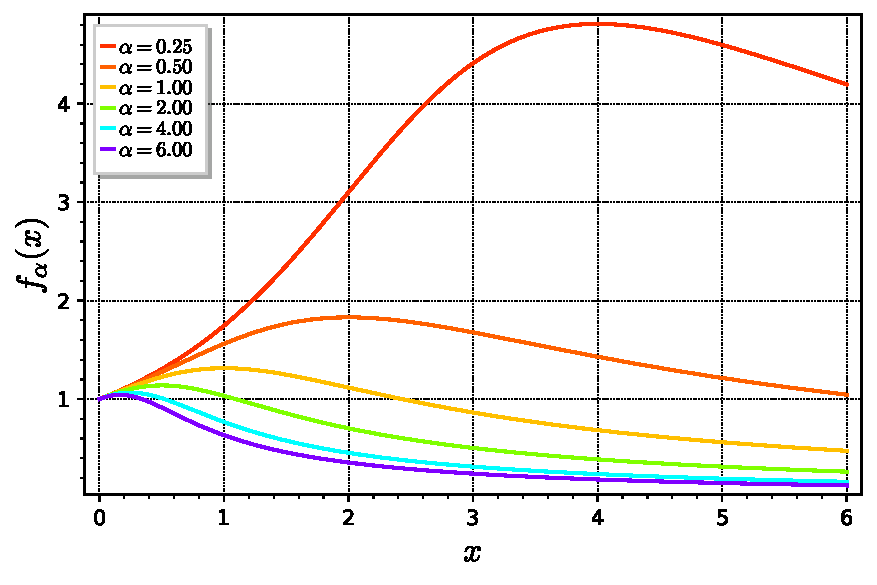
\includegraphics[width=0.6\textwidth]{vai_f_alpha_x.pdf}}
\caption[]{\label{f:vai:f_alpha_x} \footnotesize
Function $f_\alpha(x)$, defined by Eq.~(\ref{e:vai:sol_r_x_v0_small}),
for some selected values of $\alpha > 1/8$. For each value of $\alpha$, the maximum
of $f_\alpha(x)$ is achieved for $x=\alpha^{-1}$.
\textsl{[Figure generated by the notebook \ref{s:sam:Vaidya_solve_ode_out}]}
}
\end{figure}

It appears clearly on Eq.~(\ref{e:vai:eq_out_v0_small}) that
the homothety $H_\lambda:\ (t, r) \mapsto (\lambda t, \lambda r)$
transforms the geodesic $\Li_{(u,\th,\ph)}^{\rm out}$  into the geodesic
$\Li_{(u',\th,\ph)}^{\rm out}$ with $u' = u - \ln \lambda$,
in agreement with the homothetic symmetry of $(\M_{\rm rad}, \w{g})$ discussed
above.

Some outgoing radial null geodesics are depicted as solid green lines
in Fig.~\ref{f:vai:diag_S0}. In $\M_{\rm rad}$, they obey
Eq.~(\ref{e:vai:eq_out_v0_small}).
Note that the homothetic symmetry appears clearly on the figure.
If a geodesic $\Li_{(u,\th,\ph)}^{\rm out}$  has a $r$-turning point in $\M_{\rm rad}$,
it must located at $x = \alpha^{-1}$, i.e. at $t/r = \alpha^{-1} - 1$,
or equivalently at
\be \label{e:vai:r_max_out}
  t = \left( \frac{v_0}{2m} - 1 \right) r .
\ee
The above equation defines a straight line through $(t,r) = (0,0)$,
whose intersection with $\M_{\rm rad}$ is depicted by a red segment
in Fig.~\ref{f:vai:diag_S0}.
\begin{remark}
The turning point value (\ref{e:vai:r_max_out}) can be obtained
directly by setting $\D r / \D t = 0$ in Eq.~(\ref{e:vai:ODE_outgoing_null})
and using the value (\ref{e:vai:S_linear}) for $M(v)$.
\end{remark}

In the Minkowski region, the outgoing radial null geodesics are straight line
segments inclined at $+45^\circ$ in Fig.~\ref{f:vai:diag_S0}, while
in the Schwarzschild region, they are curves obeying Eq.~(\ref{e:sch:outgoing_null_geod_EF})
(with the change of notation $\ti \leftrightarrow t$).


\subsection{Black hole formation} \label{s:vai:BH_formation}

In spherical symmetry, the inspection of radial null geodesics gives
a direct access to the black hole event horizon $\Hor$.
Since we have at disposal the exact solution
(\ref{e:vai:eq_out_v0_small}) for the outgoing radial null geodesics,
let us determine the location of $\Hor$ for the homothetic
shell collapse.
We arrive at the following result:
\begin{greybox}
The homothetic imploding radiation shell with $\alpha := 2m/v_0 > 1/8$
generates a black hole. The black hole event horizon $\Hor$
is the future light cone of the point of IEF coordinates
$(t, r) = (t_{\rm hb}, 0)$, with\footnote{As in Chap.~\ref{s:lem}, the subscript `hb' stands
for \emph{horizon birth}.}
\be \label{e:vai:t_hb}
    \encadre{ t_{\rm hb} = - 4 m \exp \left[ - \frac{2}{\sqrt{8\alpha - 1}}
    \arctan\left( \frac{1}{\sqrt{8\alpha - 1}} \right) \right] } .
\ee
Outside the radiation shell, $\Hor$ coincides with the
Killing horizon of Schwarzschild spacetime located at $r=2m$.
\end{greybox}

\begin{figure}
\centerline{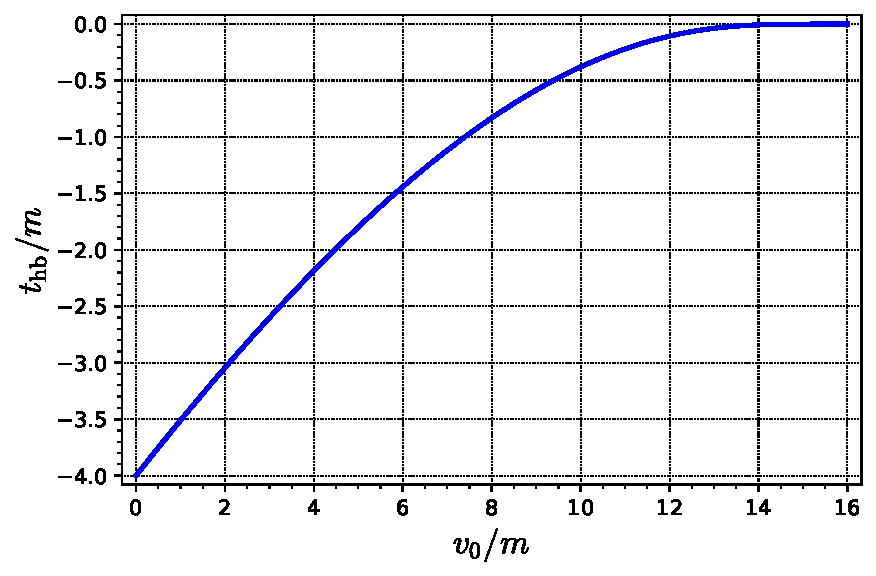
\includegraphics[width=0.6\textwidth]{vai_thb_v0.pdf}}
\caption[]{\label{f:vai:thb_v0} \footnotesize
Value $t_{\rm hb}$ of the coordinate $t$ at the black hole birth [Eq.~(\ref{e:vai:t_hb})]
as a function of the radiation shell thickness $v_0$, for
the homothetic shell collapse [Eq.~(\ref{e:vai:S_linear})].
}
\end{figure}


\begin{proof}
In the Schwarzschild region $\M_{\rm Sch}$, the Killing horizon is the hypersurface
$r = 2m$. It is generated by the null geodesics $\Li^{{\rm out},\Hor}_{(\th,\ph)}$
discussed in Sec.~\ref{s:sch:radial_null_IEF} [cf. Eq.~(\ref{e:sch:outgoing_null_geod_H})].
Let us consider one such geodesic, $\hat{\Li}$ say.
It has a fixed value of $(\th,\ph)$ and, when followed in the past direction,
it encounters the outer edge of the radiation region $\M_{\rm rad}$
(hypersurface $v=v_0$) at the point $A$ such that $r_A = 2m$ and $t_A = v_0 - 2m$
(cf. Fig.~\ref{f:vai:diag_S0}, where $\hat{\Li}$ can be identified with the
black curve). If $\hat{\Li}$ is prolonged into $\M_{\rm rad}$, still in the past direction, it encounters the inner edge of $\M_{\rm rad}$ (hypersurface $v=0$) at the point $B$
(cf. Fig.~\ref{f:vai:diag_S0}).
The portion $AB$ of $\hat{\Li}$ coincides with the geodesic $\Li_{(u_B,\th,\ph)}^{\rm out}$
of the outgoing radial null family given by Eq.~(\ref{e:vai:eq_out_v0_small}),
with $u_B = - \ln(r_B / m)$ (since $f_\alpha(x_B)=1$, given that $x_B = 0$).
We have then $r_A = r_B f_\alpha(x_A)$.
Now, by definition of $x$ [Eq.~(\ref{e:vai:def_x_v_r})] and
$\alpha$ [Eq.~(\ref{e:vai:def_alpha})],
$x_A = v_A / r_A = v_0 / (2m) = \alpha^{-1}$.
We have thus $2 m = r_B f_\alpha(\alpha^{-1})$. In view of expression
(\ref{e:vai:sol_r_x_v0_small}) for $f_\alpha(x)$, there comes
\[
    r_B = 2 m \exp \left[ - \frac{2}{\sqrt{8\alpha - 1}}
    \arctan\left( \frac{1}{\sqrt{8\alpha - 1}} \right) \right] .
\]
Since $B$ is located on the hypersurface $v=0$, we have $t_B = - r_B$.
If the radial null geodesic $\hat{\Li}$
is prolonged further to the past in the Minkowski
region $\M_{\rm Min}$, it becomes the straight line of equation $t = r - 2 r_B$.
$\hat{\Li}$ thus reaches $r=0$ at some event $C$ of
coordinate $t = t_{\rm hb} = -2 r_B$, hence Eq.~(\ref{e:vai:t_hb}).

There remains to prove that the null hypersurface generated by
$\hat{\Li}$ when $(\th,\ph)$ varies, i.e. the future light cone $\Hor$
of the point $(t, r) = (t_{\rm hb}, 0)$, is indeed the black hole event
horizon. To this aim, let us consider an outgoing radial null geodesic $\Li$
in $\M_{\rm Min}$ such that $\Li$ crosses $r=0$ at $t < t_{\rm hb}$,
i.e. outside $\Hor$.
$\Li$ arrives then at the inner edge of $\M_{\rm rad}$
with $r = r_0 > r_B$.  In $\M_{\rm rad}$,
according to Eq.~(\ref{e:vai:eq_out_v0_small}),
$\Li$ is homothetic to a part of $\hat{\Li}$ with a ratio $r_0 / r_B > 1$. It emerges
then at the outer edge of $\M_{\rm rad}$ with $r > r_A = 2 m$. It is
then in the exterior of the Schwarzschild black hole and can reach
the future null infinity $\scri^+$ of Schwarzschild spacetime.
On the contrary, if $\Li$ crosses $r=0$ with $t > t_{\rm hb}$,
i.e. inside $\Hor$,
it encounters the inner edge of $\M_{\rm rad}$ with
$r = r_0 < r_B$. A part of $\Li$ is then homothetic to the segment $BA$ of
$\hat{\Li}$ with a ratio $r_0 / r_B < 1$. Then either (i) $\Li$ has a
$r$-turning point and reaches $r=0$
in $\M_{\rm rad}$ or (ii) $\Li$ reaches
the outer edge of $\M_{\rm rad}$ ($v = v_0$) at some point $A'$.
Given that $x_A = \alpha^{-1}$ corresponds to the maximum of $f_\alpha(x)$, one
has necessarily $f_\alpha(x_{A'}) \leq f_\alpha(x_A)$ and thus
$r_0 f_\alpha(x_{A'}) < r_B f_\alpha(x_A)$. By
Eq.~(\ref{e:vai:eq_out_v0_small}), this implies $r_{A'} < r_A = 2m$, so
that $\Li$ emerges in the black hole region of Schwarzschild spacetime.
So none of the two possible cases (i) or (ii) leads to $\Li$ reaching
$\scri^+$. We conclude that $\Hor$ is a black hole
horizon.
\end{proof}

The black hole event horizon $\Hor$ is depicted as the thick black curve
in Fig.~\ref{f:vai:diag_S0}. Since $t_{\rm hb} < 0$ [cf. Eq.~(\ref{e:vai:t_hb})],
one immediately notes that
\begin{greybox}
The black hole forms in the Minkowski
region of Vaidya spacetime, i.e. in a region where the spacetime curvature
is zero.
\end{greybox}
This striking feature reflects the non-local character of black holes and
will be discussed further in Chap.~\ref{s:loc}.

The dependency of $t_{\rm hb}$
on the width $v_0$ of the radiation shell is shown in Fig.~\ref{f:vai:thb_v0}.
One has $-4m < t_{\rm hb} < 0$, with
\be \label{e:vai:limit_thb_v0_0}
    \lim_{v_0 \to 0} t_{\rm hb} = - 4m \qand
     \lim_{v_0 \to 16m} t_{\rm hb} = 0 .
\ee
\begin{remark}
The first limit in (\ref{e:vai:limit_thb_v0_0}), which corresponds to $\alpha\to +\infty$ in Eq.~(\ref{e:vai:t_hb}),
is easily recovered by a pure geometric construction: a zero-width
shell implies the equality of the two points $A$ and $B$ considered in the
proof of (\ref{e:vai:t_hb}), as well as $t_A = t_B = - 2m$, hence
$t_C = t_{\rm hb} = - 4 m$.
\end{remark}

\begin{hist}
The imploding radiation shell with $M(v)$ piecewise linear (homothetic model)
has been extensively
studied by Achilles Papapetrou\index{Papapetrou, A.} in 1985 \cite{Papap85}.
He obtained the solution (\ref{e:vai:eq_out_v0_small}) for the outgoing radial
null geodesics and determined the location of the event horizon, along
the lines presented above.
\end{hist}

\subsection{Curvature singularity} \label{s:vai:thin:sing}

The Kretschmann scalar\index{Kretschmann scalar!of Vaidya metric}
$K := R_{\mu\nu\rho\sigma} R^{\mu\nu\rho\sigma}$
(cf. Sec.~\ref{s:sch:singularities})
is computed in the notebook~\ref{s:sam:Vaidya}:
\be \label{e:vai:Kretschmann}
    K = \frac{48 M(t + r)^2}{r^6} .
\ee
$K$ is identically zero in the Minkowski region ($M(r+t) = 0$), as it should!

It diverges at $r=0$ in the radiation and Schwarzschild regions ($M(r+t) > 0$), tracing the
existence of a curvature singularity there.
In other words:
\begin{greybox}
The Vaidya shell collapse introduced in Sec.~\ref{s:vai:imploding_shell}
generates a spacetime with a curvature singularity
located at $r=0$ and $t \geq 0$.
\end{greybox}

\begin{remark}
The Kretschmann scalar of Vaidya metric has the same structural form
as that of the Schwarzschild metric, compare Eq.~(\ref{e:sch:value_Kretschmann}),
while a priori $K$ could have
contained some term involving the derivative of $M(v)$. Indeed $M'(v)$
appears in some components of the Riemann tensor, since it is present in the
components of the Ricci tensor, as given by Eq.~(\ref{e:vai:Ricci_tensor}).
\end{remark}

\begin{remark}
Since the Ricci tensor of the Vaidya metric is not identically zero
[cf. Eq.~(\ref{e:vai:Ricci_tensor})], other curvature invariants that one might
have think of in order to track the curvature singularity are the Ricci scalar $R := g^{\mu\nu} R_{\mu\nu}$
and the Ricci ``squared'' $R_{\mu\nu} R^{\mu\nu}$. However, they are both identically zero
for $\w{k}$ is a null vector.
\end{remark}

The curvature singularity is depicted as the orange broken line in Fig.~\ref{f:vai:diag_S0}.
It is clear on this figure that the singularity bounds the future of both ingoing and outgoing radial null geodesics.
This will be shown rigorously in Sec.~\ref{f:vai:thin_CP}.
This implies that the curvature singularity is spacelike, as in Schwarzschild spacetime.

For the homothetic collapse with $v_0 < 16\, m$ considered in Secs.~\ref{s:vai:sol_M_linear} and
\ref{s:vai:BH_formation}, one has $t_{\rm hb} < 0$ [Eq.~(\ref{e:vai:t_hb})], so that
the curvature singularity is entirely located in the black hole region. It is therefore hidden
from a remote observer. In Sec.~\ref{s:vai:naked_sing}, we will see that this is no longer the
case for $v_0 > 16 m$: the singularity is then naked.

\subsection{Trapped surfaces} \label{s:vai:trapped_surf}

Let us show that there exist trapped surfaces (cf. Sec.~\ref{s:neh:trapped_surfaces}) in the
radiation and Schwarzschild regions of Vaidya spacetime.
To this aim, we consider a 2-surface $\Sp$ defined by $(t,r) = \mathrm{const}$. It is a closed surface
with the topology of a 2-sphere, spanned by the coordinates $(\th,\ph)$.
Moreover, $\Sp$ is spacelike since the metric induced by $\w{g}$ on it  is
$\w{q} = r^2 \left( \dd\th^2 + \sin^2\th\, \dd\ph^2 \right) $, as readily seen
on Eq.~(\ref{e:vai:metric_IEF}). The area of $\Sp$ is simply $4\pi r^2$
($r$ is the areal radius coordinate), so to check whether $\Sp$ is a trapped surface,
it suffices to determine the behavior
of $r$ along the two null directions normal to $\Sp$, which are nothing but
the directions of the ingoing and outgoing radial null geodesics.
Along the ingoing geodesics (tangent vector $\w{k}$),
one has $\D r / \D t = - 1$, since $\w{k} = \wpar_t - \wpar_r$ [Eq.~(\ref{e:vai:k_IEF})],
so that the expansion is negative: $\theta_{(\w{k})} < 0$.
Along the outgoing radial null geodesics, $\D r / \D t$ is given by Eq.~(\ref{e:vai:ODE_outgoing_null}).
The sign of the expansion $\theta_{(\wl)}$ is then that of $r - 2M(t+r)$. Hence
\begin{greybox}
The spherically symmetric surface $\Sp$ defined by $(t,r) = \mathrm{const}$ obeys
\be \label{e:vai:S_trapped}
    \Sp \text{ is trapped} \iff r < 2M(t+r) .
\ee
Obviously, the above criterion cannot be fulfilled in the Minkowski region, where $M(t+r) = 0$.
On the contrary, trapped surfaces exist
in the central part of the radiation region, since $M(t+r) > 0$ there.
They also exist in the black hole part ($r < 2m$)
of the Schwarzschild region, where
$M(t+r) = m$.
\end{greybox}

The set formed by all the marginally trapped spheres
of fixed $(t,r)$
is the hypersurface $\mathscr{T}$ defined by $\theta_{(\wl)} = 0$.
Its equation is obtained by saturating the inequality
in Eq.~(\ref{e:vai:S_trapped}):
\be \label{e:vai:def_T}
    \mathscr{T}:\qquad r = 2M(t + r).
\ee
As we shall see in
Chap.~\ref{s:loc}, $\mathscr{T}$ is called a
\defin{future outer trapping horizon}\index{future!outer trapping horizon}\index{trapping horizon!future!outer --}.
We have the following characterization of $\mathscr{T}$, which follows directly
from Eq.~(\ref{e:vai:def_T}) implying $\D r / \D t = 0$ in Eq.~(\ref{e:vai:ODE_outgoing_null}):
\begin{greybox}
If an outgoing radial null geodesic $\Li$ crosses $\mathscr{T}$,
the crossing point is a $r$-turning point of $\Li$.
\end{greybox}
This feature appears clearly in Figs.~\ref{f:vai:diag_S0} and \ref{f:vai:diag_S2}.
Furthermore, $\mathscr{T}$ obeys the following properties.
\begin{greybox}
In the radiation region, the future outer trapping horizon $\mathscr{T}$ is a
spacelike hypersurface, while in the Schwarzschild region, $\mathscr{T}$
coincides with the event horizon $\Hor$ (and hence is a null hypersurface).
\end{greybox}
\begin{proof}
Let us consider $(v,\th,\ph)$ as coordinates on the 3-manifold $\mathscr{T}$.
We may rewrite Eq.~(\ref{e:vai:def_T}) for $\mathscr{T}$ as $r = 2M(v)$, so that
$\dd r = 2M'(v) \, \dd v$ along $\mathscr{T}$.
Plugging this relation, as well as $2M(v)/r=1$, into Eq.~(\ref{e:vai:Vaidya_metric_null})
yields immediately the metric $\w{h}$ induced by $\w{g}$ on $\mathscr{T}$:
$\w{h} = 4 M'(v) \, \dd v^2
        + r^2 \left( \dd\th^2 + \sin^2\th\, \dd\ph^2 \right)$.
In $\M_{\rm rad}$, $M'(v) > 0$ [cf. Eq.~(\ref{e:vai:mass_function})], which
implies that $\w{h}$ is a positive definite metric. Hence $\mathscr{T}$
is a spacelike hypersurface in $\M_{\rm rad}$. In $\M_{\rm Sch}$, $M'(v) = 0$ and $\w{h}$
is a degenerate metric, so that $\mathscr{T}$ is a null hypersurface there.
Actually, in $\M_{\rm Sch}$, Eq.~(\ref{e:vai:def_T}) reduces
to $r = 2m$, so that $\mathscr{T}$ coincides with the event horizon $\Hor$ there.
\end{proof}

\begin{remark}
The spacelike character of $\mathscr{T}$ is actually a generic feature of future outer trapping horizons in non-stationary spacetimes (such as $(\M_{\rm rad},\w{g})$),
as we shall see in Chap.~\ref{s:loc}.
\end{remark}

\begin{figure}
\centerline{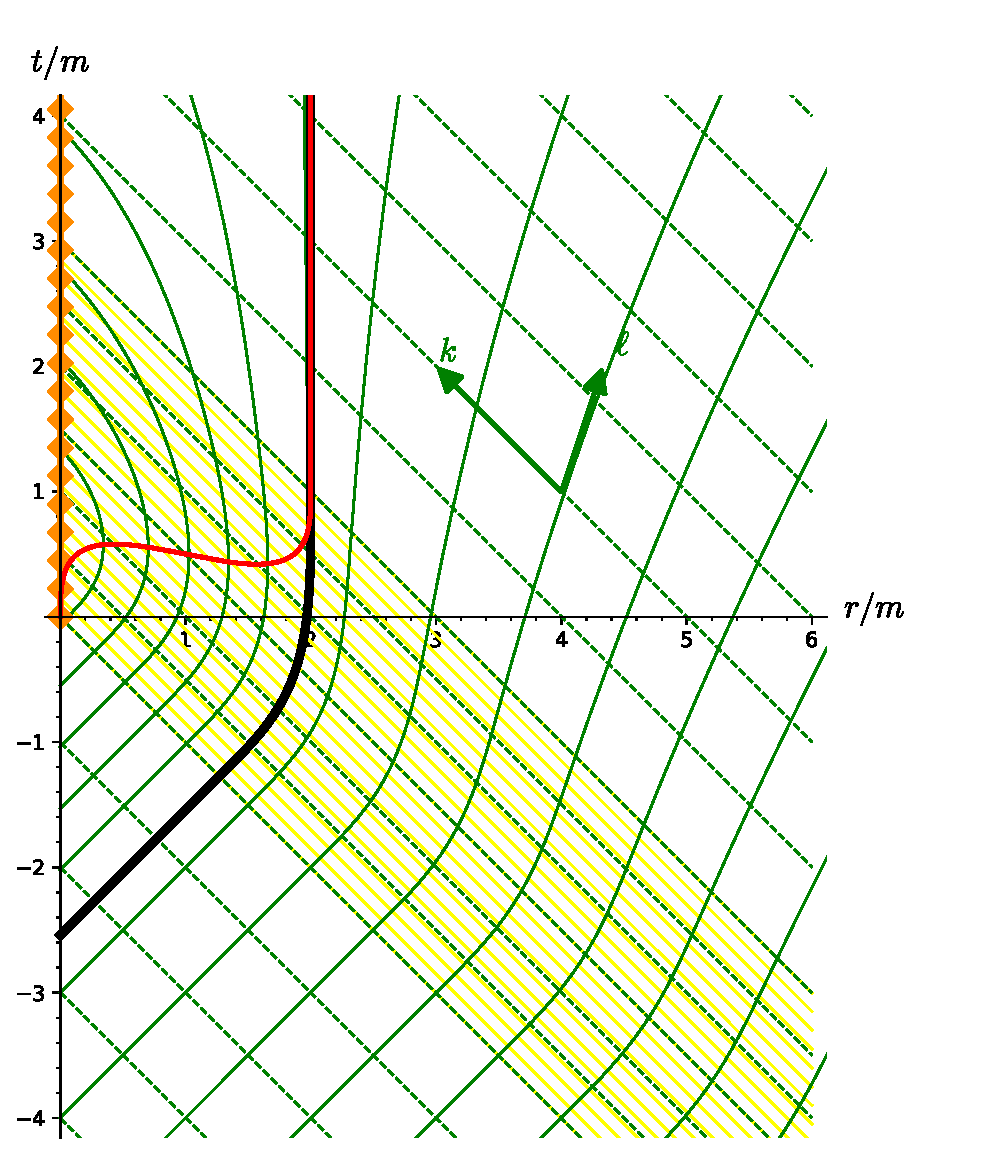
\includegraphics[width=0.6\textwidth]{vai_diag_S2.pdf}}
\caption[]{\label{f:vai:diag_S2} \footnotesize
Same as Fig.~\ref{f:vai:diag_S0}, but for the $C^2$ mass function $M(v)$
corresponding to the choice $S(x) = 6 x^5 - 15 x^4 + 10 x^3$
in Eq.~(\ref{e:vai:mass_function}) (cf. the red curve in Fig.~\ref{f:vai:mass_function}).
Note that the trapping horizon $\mathscr{T}$
(red curve) is tangent to the event horizon $\Hor$ (black curve) at the
outer edge of radiation region ($(t, r) = (m, 2m)$).
\textsl{[Figure generated by the notebook \ref{s:sam:Vaidya}]}
}
\end{figure}

For the homothetic shell model considered in Sec.~\ref{s:vai:sol_M_linear},
$M(v) = m v / v_0 = \alpha v / 2$ and the equation of
$\mathscr{T}$ in $\M_{\rm rad}$ is vey simple:
\be \label{e:vai:def_T_hom}
    \mathscr{T} \cap \M_{\rm rad}:\qquad r = \alpha v .
\ee

\begin{example}
For $v_0 = 3m$, as in Fig.~\ref{f:vai:diag_S0},
$\alpha = 2/3$ and we get $r = 2v/3 = 2(t+r)/3$ or equivalently $t = r / 2$. Hence, in $\M_{\rm rad}$,
$\mathscr{T}$ appears as the straight line segment of slope $1/2$
drawn in red in Fig.~\ref{f:vai:diag_S0}.
It appears clearly there that the outgoing radial null geodesics
that cross $\mathscr{T}$ do it at a $r$-turning point.
By considering the light cones delineated by the ingoing and outgoing radial null geodesics, it
also appears
clearly on Fig.~\ref{f:vai:diag_S0} that $\mathscr{T}$ is a spacelike hypersurface in $\M_{\rm rad}$.
\end{example}

\begin{remark}
As shown above, $\mathscr{T}$ coincides with $\Hor$ in $\M_{\rm Sch}$, so that
the slope of $\mathscr{T}$ in Fig.~\ref{f:vai:diag_S0} changes abruptly from $1/2$
to $+\infty$ at the outer edge of $\M_{\rm rad}$.
This lack of smoothness of the hypersurface $\mathscr{T}$ reflects actually
the lack of smoothness of the function $M(v)$ of the homothetic shell model
(cf. the blue curve in Fig.~\ref{f:vai:mass_function}). Would $M(v)$ be smooth,
$\mathscr{T}$ would merge smoothly with $\Hor$ at $v=v_0$. This is shown in
Fig.~\ref{f:vai:diag_S2}, where $M(v)$ is of class $C^2$. Besides, we can check
on this figure that, while it has a shape more complicated
that in Fig.~\ref{f:vai:diag_S0}, $\mathscr{T}$ always lies outside the null cones in
$\M_{\rm rad}$, i.e. is a spacelike hypersurface there.
\end{remark}

\subsection{Carter-Penrose diagram} \label{f:vai:thin_CP}

In order to draw a Carter-Penrose diagram of the Vaidya collapse,
we need first to introduce a double-null coordinate system $(u, v, \th,\ph)$
in the radiation region $\M_{\rm rad}$, i.e. a coordinate system such that
$u$ is constant along the outgoing radial null geodesics ---
$v$ being constant along the ingoing ones by construction.
For the homothetic model ($M(v) = \alpha v /2$ in $\M_{\rm rad}$),
the relation between coordinates $(u, v, \th,\ph)$ and
$(v, r, \th, \ph)$ is provided by Eq.~(\ref{e:vai:eq_out_v0_small}):
\be \label{e:vai:u_lnr_v}
    \encadre{ u = - \ln\left(\frac{r}{m}\right) + \ln f_\alpha\left(\frac{v}{r}\right) }.
\ee
From Eqs.~(\ref{e:vai:u_lnr_v}) and (\ref{e:vai:lnf_alpha}), we get
\[
   \dd u = - \frac{1}{r} \dd r  +  \frac{1 - \alpha x}{\alpha x^2 - x + 2} \dd\left(\frac{v}{r}\right)
    = - \frac{1}{r(\alpha x^2 - x + 2)} \left[ (\alpha x - 1) \dd v + 2 \dd r \right] .
\]
By comparing with (\ref{e:vai:self_similar_metric}), we deduce immediately
the expression of the metric tensor in terms of the coordinates $(u,v,\th,\ph)$:
\be \label{e:vai:thin:g_uv}
    \w{g} =  - r(\alpha x^2 - x + 2) \, \dd u \, \dd v
    + r^2 \left( \dd\th^2 + \sin^2\th\, \dd\ph^2 \right) \qquad
        (0 \leq v \leq v_0) ,
\ee
where $x := v/r$  and $r$ is to be considered as a function of $(u,v)$ defined implicitly
by Eq.~(\ref{e:vai:u_lnr_v}).
Since for $\alpha > 1/8$, the polynomial $\alpha x^2 - x + 2$ never vanishes,
the metric component $g_{uv}$ read on Eq.~(\ref{e:vai:thin:g_uv}) is
nonzero in all $\M_{\rm rad}$. This shows that
the coordinates $(u,v,\th,\ph)$ are regular on $\M_{\rm rad}$
(except for the singularities inherent to the spherical coordinates $(\th,\ph)$).
Moreover, they constitute a \defin{double-null coordinate system}\index{double-null coordinates}:
we read on Eq.~(\ref{e:vai:thin:g_uv}) that
$g_{uu} = 0$ and $g_{vv} = 0$, which means that the coordinate vectors $\wpar_u$
and $\wpar_v$ are both null. The vector $\wpar_u$ is actually tangent to the
ingoing radial null geodesics $\Li^{\rm in}_{(v,\th,\ph)}$
and the vector $\wpar_v$ is tangent to the outgoing ones, $\Li^{\rm out}_{(u,\th,\ph)}$.
Furthermore, the null vectors $\wpar_u$
and $\wpar_v$ are both future-directed. Indeed,
the time orientation of Vaidya spacetime is given by the vector $\w{k}$
(cf. Sec.~\ref{s:vai:general}) and we deduce from Eq.~(\ref{e:vai:k_d_dr})
that $\w{k} = - (\dert{u}{r}) \, \wpar_u$. Evaluating $\dert{u}{r}$
from Eqs.~(\ref{e:vai:u_lnr_v}) and (\ref{e:vai:lnf_alpha}), we get
\be
    \w{k} = \frac{2}{r(\alpha x^2 - x + 2)}\, \wpar_u .
\ee
The coefficient in front of $\wpar_u$ being always positive, we conclude that
$\wpar_u$ is future-directed. Then, from Eq.~(\ref{e:vai:thin:g_uv}),
$\w{g}(\wpar_u,\wpar_v) = g_{uv} < 0$, so that, according to Lemma~2 of
Sec.~\ref{s:fra:time_orientation}, $\wpar_v$ is future-directed as well.

\begin{remark}
The reader may have noticed a slight asymmetry between the coordinates $u$
and $v$: $u$ is dimensionless, while $v$ has the dimension of a time. We could
of course make $u$ have the same dimension as $v$ by introducing an overall
factor $m$ in the right-hand side of Eq.~(\ref{e:vai:u_lnr_v}). However, this
would make the formulas slightly more complicate, without any real
benefit.
\end{remark}

Let us discuss the boundary of $\M_{\rm rad}$ in terms of the $(u,v)$ coordinates.
By definition of $\M_{\rm rad}$, a part of the boundary consists in the
hypersurfaces $v=0$ and $v = v_0$. Another part corresponds to the limit
$r\to +\infty$. In view of Eq.~(\ref{e:vai:u_lnr_v}) and $f_\alpha(0) = 1$
(cf. Eq.~(\ref{e:vai:lnf_alpha}) or Fig.~\ref{f:vai:f_alpha_x}), this corresponds
to $u  \to -\infty$. The last part of the boundary of $\M_{\rm rad}$
is set by the curvature singularity at $r=0$ (cf. Sec.~\ref{s:vai:thin:sing}). Taking
the limit $r \to 0$ in Eq.~(\ref{e:vai:u_lnr_v}), we found the equation ruling
this boundary in terms of $(u,v)$:
\be \label{e:vai:thin:r_0_uv}
    u = \ln\left( \frac{v_0}{v} \right) + u_0, \qquad
    u_0 := \ln \sqrt{\frac{\alpha}{2}}
        + \frac{1}{\sqrt{8\alpha - 1}} \left[
    \frac{\pi}{2}
    + \arctan\left( \frac{1}{\sqrt{8\alpha - 1}} \right)\right] .
\ee
We conclude that the range of the coordinates $(u,v)$ on $\M_{\rm rad}$ is
(cf. Fig.~\ref{f:vai:thin_double_null})
\be
    \M_{\rm rad}: \quad \left\{ \begin{array}{l}
    0 \leq v \leq v_0 \\
    -\infty < u <  \ln\left( \frac{v_0}{v} \right) + u_0 .
    \end{array} \right.
\ee
In the last inequality, the right-hand side must be replaced by $+\infty$ if $v=0$.

\begin{figure}
\centerline{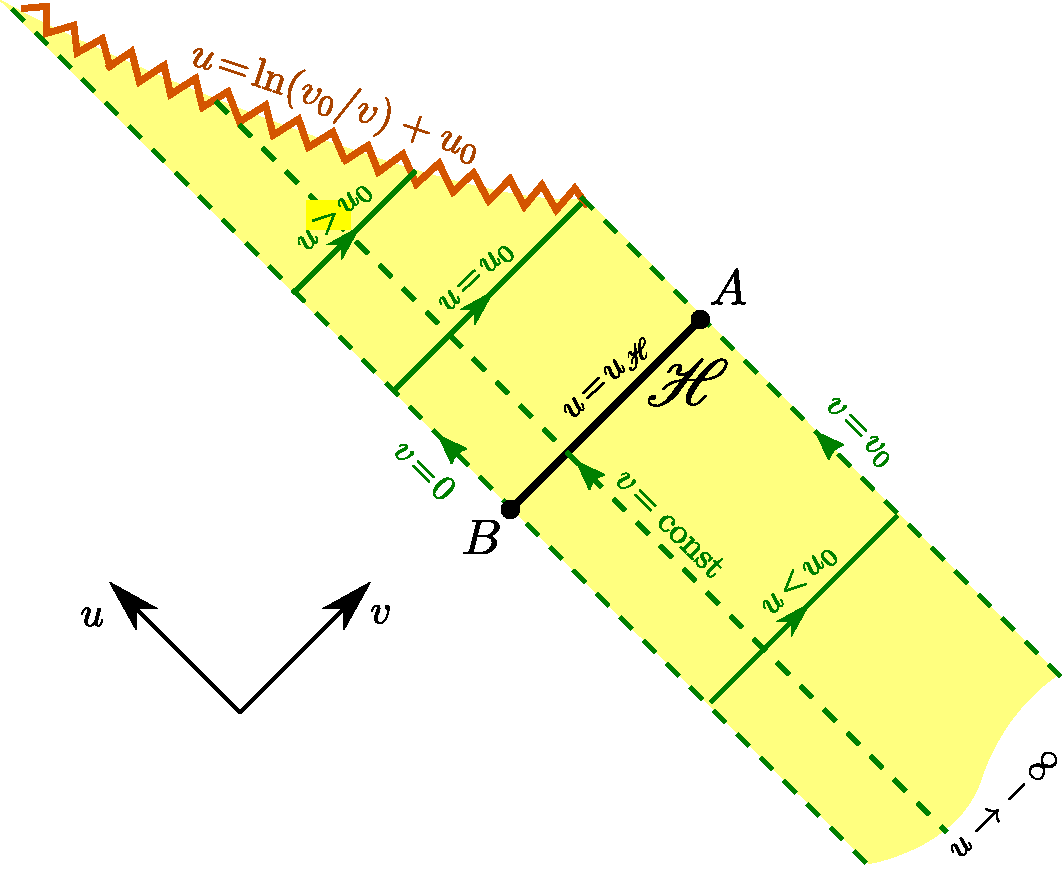
\includegraphics[width=0.6\textwidth]{vai_thin_double_null.pdf}}
\caption[]{\label{f:vai:thin_double_null} \footnotesize
Radiation region $\M_{\rm rad}$ for the homothetic model ($M(v) = m v/v_0$) with $v_0 < 16m$,
depicted in terms of the double-null coordinates
$(u, v)$. Solid (resp. dashed) green lines are outgoing (resp. ingoing)
radial null geodesics. The orange zigzag curve corresponds to the curvature
singularity at $r=0$.
The black segment marks the event horizon $\Hor$, while the red curve marks the trapping horizon
$\mathscr{T}$ [Eq.~(\ref{e:vai:thin:trap_uv})].
The points $A$ and $B$ are the same as in Fig.~\ref{f:vai:diag_S0}.
}
\end{figure}



Along a given ingoing radial null geodesic $\Li^{\rm in}_{(v,\th,\ph)}$,
$u$ can be considered as a (non-affine) parameter, $\wpar_u$
being tangent to $\Li^{\rm in}_{(v,\th,\ph)}$. The geodesic hits the curvature
singularity for $u \to \ln(v_0/v) + u_0$.
Regarding an outgoing radial null geodesic $\Li^{\rm out}_{(u,\th,\ph)}$,
$v$ can be considered as a (non-affine) parameter, $\wpar_v$
being tangent to $\Li^{\rm out}_{(u,\th,\ph)}$. If $u < u_0$,
$\Li^{\rm out}_{(u,\th,\ph)}$ reaches the outer boundary of the radiation
shell for $v=v_0$ and is extendible to a null geodesic of the Schwarzschild
region, while if $u \geq u_0$, $\Li^{\rm out}_{(u,\th,\ph)}$ hits the
curvature singularity for $v \to v_0 \mathrm{e}^{u_0 - u}$
(cf. Fig.~\ref{f:vai:thin_double_null}).

The event horizon $\Hor$ crosses $\M_{\rm rad}$ at a fixed value of $u$, $u_\Hor$ say,
since it is generated by outgoing null geodesics. The value of $u_\Hor$ is found
by setting $r=2m$ and $v=v_0$ in Eq.~(\ref{e:vai:u_lnr_v}):
\be \label{e:vai:thin:u_H}
    u_\Hor = \frac{2}{\sqrt{8\alpha - 1}}\arctan\left( \frac{1}{\sqrt{8\alpha - 1}}\right)
    - \ln 2 .
\ee
Given expression
(\ref{e:vai:thin:r_0_uv}) for $u_0$, it is easy to check that $u_\Hor < u_0$,
as drawn in Fig.~\ref{f:vai:thin_double_null}.


\begin{figure}
\centerline{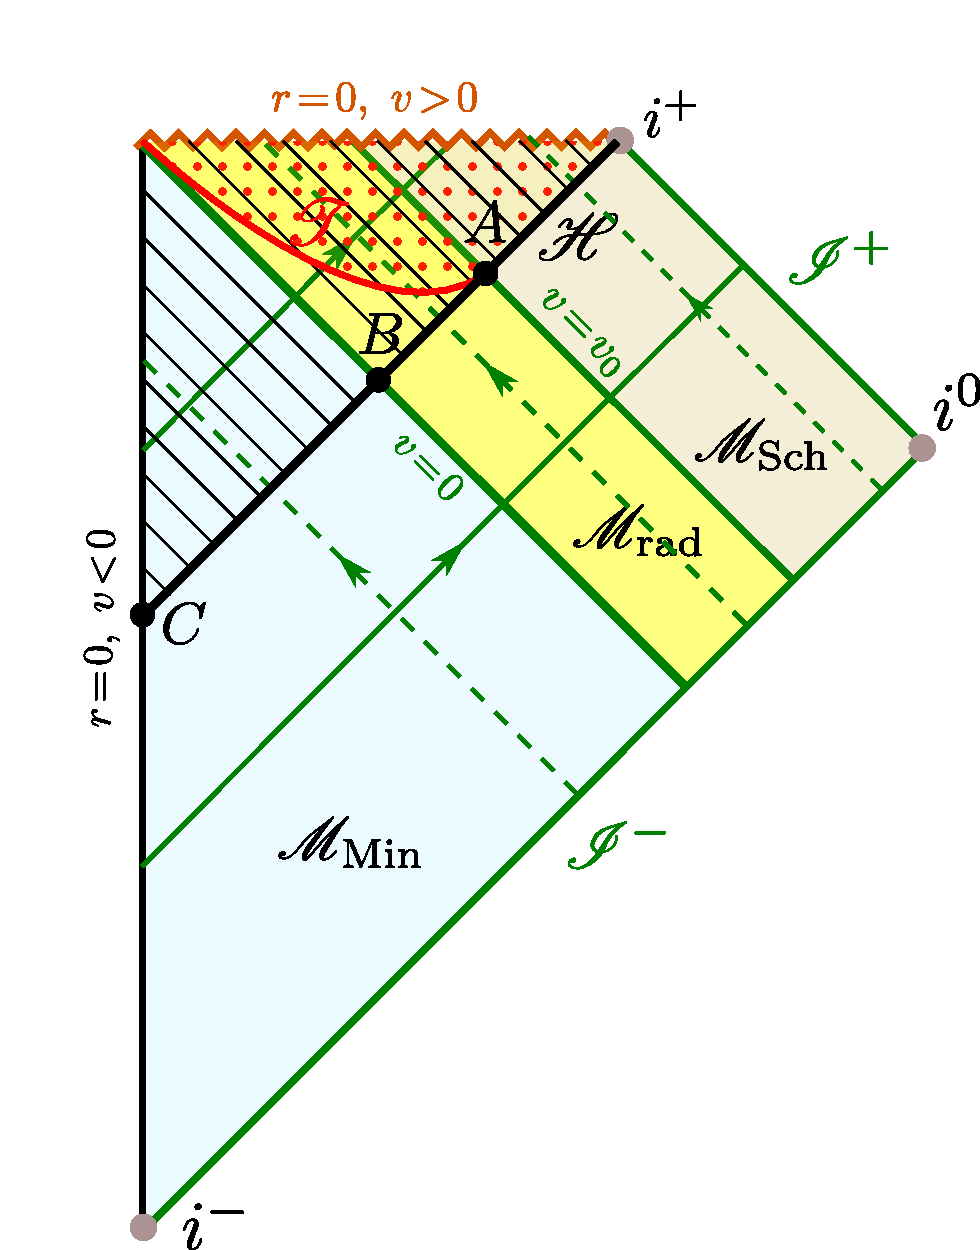
\includegraphics[width=0.45\textwidth]{vai_CPdiag_thin.pdf}}
\caption[]{\label{f:vai:CPdiag_thin} \footnotesize
Carter-Penrose diagram of Vaidya collapse
for the homothetic shell model ($M(v) = m v/v_0 = \alpha v /2$) with
$\alpha > 1/8$ ($v_0 < 16m$).
The Minkowski region $\M_{\rm Min}$, radiation region $\M_{\rm rad}$
and Schwarzschild region $\M_{\rm Sch}$ are depicted in respectively
pale blue, yellow and grey.
Solid (resp. dashed) green lines are outgoing (resp. ingoing)
radial null geodesics.
The orange zigzag segment corresponds to the curvature
singularity at $r=0$. The hatched area is the black hole region,
delimited by the event horizon $\Hor$.
The red dot-filled area, delimited by the future outer trapping horizon
$\mathscr{T}$ (red curve),
is the region where the spheres $(t,r)=\mathrm{const}$
are trapped surfaces.
The points $A$, $B$ and $C$ along $\Hor$ are the same as in Fig.~\ref{f:vai:diag_S0}.
}
\end{figure}

Regarding the future outer trapping horizon $\mathscr{T}$ introduced in
Sec.~\ref{s:vai:trapped_surf}, it obeys $r=\alpha v$ in $\M_{\rm rad}$
[Eq.~(\ref{e:vai:def_T_hom})],
so that the equation
of $\mathscr{T}$ in terms of the double-null coordinates is easily obtained
by substituting $\alpha^{-1}$ for $v/r$ in Eq.~(\ref{e:vai:u_lnr_v})
and making use of expressions (\ref{e:vai:sol_r_x_v0_small}) and (\ref{e:vai:thin:u_H}); one gets
\be \label{e:vai:thin:trap_uv}
  \mathscr{T}: \qquad  u = \ln\left( \frac{v_0}{v} \right) + u_\Hor .
\ee
Note that this implies $u\to +\infty$ for $v\to 0$ and $u\to u_\Hor$
for $v\to v_0$; the latter property agrees with $\mathscr{T}$ coinciding
with $\Hor$ in $\M_{\rm Sch}$, i.e. for $v > v_0$.
$\mathscr{T}$ is drawn as a red curve in Fig.~\ref{f:vai:thin_double_null}.

The spacetime diagram of $\M_{\rm rad}$ in Fig.~\ref{f:vai:thin_double_null}
is already conformal since all radial null geodesics are straight lines
inclined at $\pm 45^\circ$. To integrate it into a Carter-Penrose diagram,
one needs to compactify it along the $u$ direction by introducing a
coordinate of the type $U = \arctan u$ --- the $v$ direction begin already
compactified, given the finite range of $v$ in $\M_{\rm rad}$.
One can then match the obtained diagram to
Carter-Penrose diagrams of $\M_{\rm Min}$ (cf. Fig.~\ref{f:glo:conf_Mink_null})
and $\M_{\rm Sch}$ (cf. Fig.~\ref{f:max:carter-penrose-std} or \ref{f:max:carter-penrose-FN})
to get a Carter-Penrose diagram of the whole Vaidya spacetime, as shown
in Fig.~\ref{f:vai:CPdiag_thin}.

\begin{hist}
The double-null coordinates $(u,v)$, leading to expression (\ref{e:vai:thin:g_uv}) of the
metric tensor in $\M_{\rm rad}$, have been introduced by
B. Waugh\index{Waugh, B.} and Kayll Lake\index{Lake, K.} in 1986 \cite{WaughL86}.
A Carter-Penrose diagram similar to that of Fig.~\ref{f:vai:CPdiag_thin} except
for the radiation region extending to $\scri^+$ (no pure Schwarzschild exterior but
$M'(v) \to 0$ for $v\to +\infty$) has been exhibited by Yuhji Kuroda\index{Kuroda, Y.}
in 1984 \cite{Kurod84} (cf. his Fig. 2b).
The case of a radiation region bounded by $v = v_0$, as here, can be found in Fig.~2 of a 2007 article by
Brien C. Nolan\index{Nolan, B.C} \cite{Nolan07}.
\end{hist}


%%%%%%%%%%%%%%%%%%%%%%%%%%%%%%%%%%%%%%%%%%%%%%%%%%%%%%%%%%%%%%%%%%%%%%%%%%%%%%%

\section{Configurations with a naked singularity} \label{s:vai:naked_sing}

\subsection{The low radiation density case} \label{s:vai:low_alpha}

In Sec.~\ref{s:vai:infall}, we have focused on homothetic radiation shells
($M(v) = \alpha v / 2$) with
$\alpha > 1/8$ [Eq.~(\ref{e:vai:v0_small})].
Let us now discuss the opposite case\footnote{The marginal case $\alpha = 1/8$
will not be discussed here; it is actually qualitatively similar to the
case $\alpha < 1/8$ insofar as it leads to a naked singularity as well \cite{Papap85}.}:
\be \label{e:vai:v0_large}
    \alpha < \frac{1}{8} \iff v_0 > 16 \, m .
\ee
In view of the form (\ref{e:vai:T_alpha}) of the energy momentum tensor, this
corresponds to a low energy density of the radiation field. When (\ref{e:vai:v0_large})
is fulfilled, the polynomial $P_\alpha(x) := \alpha x^2 - x + 2$, which appears in the
numerator of the ODE (\ref{e:vai:ODE_outgoing_x}) ruling outgoing radial null geodesics
in $\M_{\rm rad}$,
admits two real roots:
\be \label{e:vai:x1_x2}
    x_1 := \frac{1 - \sqrt{1 - 8\alpha}}{2\alpha}
    \qand
    x_2 := \frac{1 + \sqrt{1 - 8\alpha}}{2\alpha} .
\ee
Useful identities are $x_1 + x_2 = \alpha^{-1}$ and $x_1 x_2 = 2\alpha^{-1}$.
Note also that $2 < x_1 < 4 < x_2 < \alpha^{-1}$.
Equation~(\ref{e:vai:ODE_outgoing_x}) can be recast as
\be \label{e:vai:ODE_outgoing_x_naked}
    r \frac{\D x}{\D r} = \frac{(x - x_1)(x - x_2)}{x_1 + x_2 - x} .
\ee
This differential equation admits two special solutions, corresponding
to outgoing radial null geodesics with constant value of $x$:
\be
    x = x_1  \qand x = x_2 .
\ee
Let us denote these geodesics by respectively
$\Li^{*1}_{(\th,\ph)}$ and $\Li^{*2}_{(\th,\ph)}$.
Since $x := v/r = 1 + t/r$, their equations in terms of the IEF
coordinates $(t, r, \th, \ph)$ and in $\M_{\rm rad}$ is simply
\be
    \Li^{*1}_{(\th,\ph)}: \quad t = (x_1 - 1)r
    \qand
    \Li^{*2}_{(\th,\ph)}: t = (x_2 - 1) r.
\ee
Thus, in $\M_{\rm rad}$,
$\Li^{*1}_{(\th,\ph)}$ and $\Li^{*2}_{(\th,\ph)}$ are straight line segments
through the origin $(t, r) = (0,0)$. They are depicted
as the segments $OC$ and $OB$ respectively in Fig.~\ref{f:vai:diag_naked_S0}.

\begin{greybox}
When $(\th,\ph)$ varies, $\Li^{*1}_{(\th,\ph)}$ and $\Li^{*2}_{(\th,\ph)}$
generate null hypersurfaces, $\Hor_1$ and $\Hor_2$ respectively,
such that the homothetic Killing vector $\w{\xi}$
[cf. Eq.~(\ref{e:vai:hom_Killing})] is normal to them
in the radiation region. One says that $\Hor_1$ and $\Hor_2$
are
\defin{homothetic Killing horizons}\index{homothetic!Killing!horizon}\index{Killing!horizon!homothetic --}\footnote{Recall from Sec.~\ref{s:neh:def_Killing_hor} that
a \emph{Killing horizon} is a null hypersurface such that a Killing vector is normal to it.}.
\end{greybox}
\begin{proof}
Their equations being $t=(x_1 - 1)r$ and $t=(x_2 - 1)r$, $ \Li^{*1}_{(\th,\ph)}$ and
$ \Li^{*2}_{(\th,\ph)}$ are clearly orbits of the
homothety group $(H_\lambda)_{\lambda\in \R_{>0}}$ discussed in Sec.~\ref{s:vai:sol_M_linear}.
The group generator $\w{\xi}$ is thus tangent to the null curves $\Li^{*1}_{(\th,\ph)}$ on $\Hor_1$
and $\Li^{*2}_{(\th,\ph)}$ on $\Hor_2$. Hence,
$\w{\xi}$ is null there. Given that the
only null direction in a null hypersurface is the normal one, we conclude
that  $\w{\xi}$ is normal to $\Hor_1$ and $\Hor_2$.
\end{proof}

\begin{figure}
\centerline{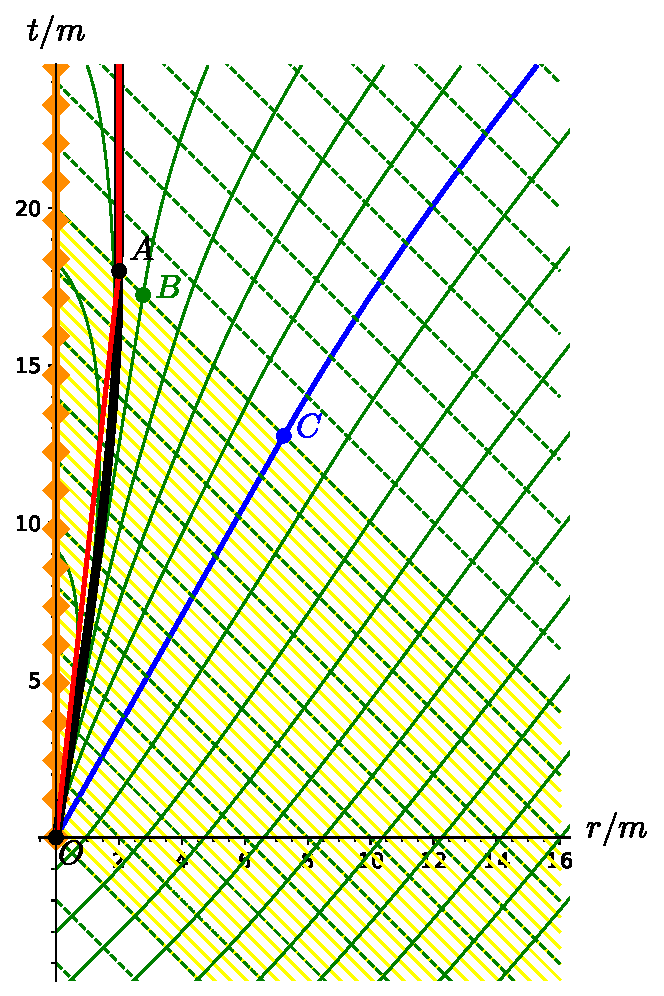
\includegraphics[width=0.6\textwidth]{vai_diag_naked_S0.pdf}}
\caption[]{\label{f:vai:diag_naked_S0} \footnotesize
Spacetime diagram of the Vaidya collapse based on the IEF coordinates $(t, r)$
and for the linear mass function $M(v)=m v/v_0$ with $v_0 = 18\, m$
(homothetic shell model with $\alpha = 1/9$,
which corresponds to $x_1 = 3$ and $x_2 = 6$).
The legend is the same as in Fig.~\ref{f:vai:diag_S0}, with in addition
the blue line marking the Cauchy horizon $\Hor_{\rm C}$ induced by the naked singularity
at $(t,r) = (0,0)$ (Sec.~\ref{s:vai:nak_Cauchy}).
In the radiation region, the straight line segments
$OB$ and $OC$ are the traces in the $(t,r)$ plane of the homothetic Killing horizons $x=x_2$ and $x=x_1$, the last one being a
part of the Cauchy horizon.
\textsl{[Figure generated by the notebook \ref{s:sam:Vaidya}]}
}
\end{figure}

Let us now consider \emph{generic} outgoing radial null geodesics, i.e.
geodesics with
$x\neq x_1$ and $x \neq x_2$; we may then rewrite Eq.~(\ref{e:vai:ODE_outgoing_x_naked}) as
\[
    \D \ln r = \frac{x_1 + x_2 - x}{(x - x_1)(x - x_2)} \, \D x .
\]
This equation is easily integrated to
\be \label{e:vai:sol_r_x_out_naked}
   \encadre{ r = c \, \frac{| x - x_2 | ^{x_1/(x_2 - x_1)}}{| x - x_1 | ^{x_2/(x_2 - x_1)}} },
\ee
where $c$ is constant along the considered geodesic.

\begin{example} \label{x:vai:sol_out_1o9}
For $\alpha=1/9$, one has $x_1 = 3$ and $x_2 = 6$ [cf. Eq.~(\ref{e:vai:x1_x2})]
and Eq.~(\ref{e:vai:sol_r_x_out_naked}) reduces to
$r = c |x - 6|/(x - 3)^2$. Such a function of $x$ is
plotted in Fig.~\ref{f:vai:r_x_naksing}.
\end{example}

\begin{figure}
\centerline{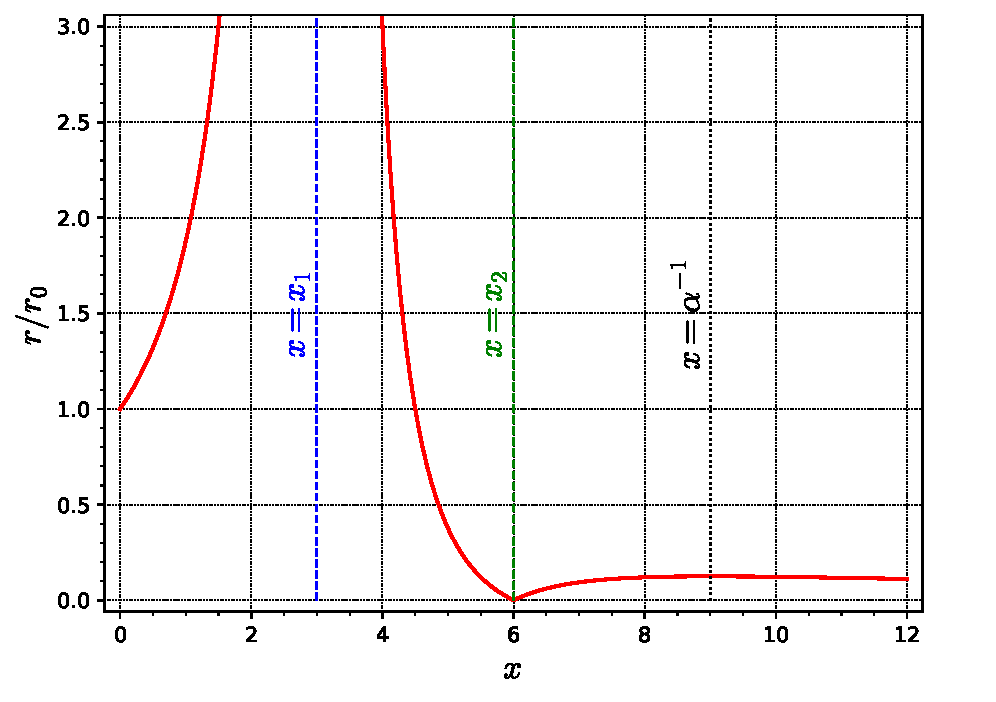
\includegraphics[width=0.6\textwidth]{vai_r_x_naksing.pdf}}
\caption[]{\label{f:vai:r_x_naksing} \footnotesize
The coordinate $r$ as a function of $x:=v/r$ along outgoing radial
null geodesics for the homothetic Vaidya collapse with
$\alpha = 1/9$ (which implies $x_1 = 3$ and $x_2 = 6$).
The graph of $r(x)$ admits a local
maximum for $x=\alpha^{-1}$, i.e. $x=9$ in the present case, although this
is barely noticeable on the figure.
\textsl{[Figure generated by the notebook \ref{s:sam:Vaidya_solve_ode_out}]}
}
\end{figure}

Having determined the outgoing radial null geodesics, we are in position to establish
the following results:
\begin{greybox}
The homothetic imploding radiation shell with $\alpha := 2m/v_0 < 1/8$
generates a black hole, the event horizon of which originates
at $(t,r) = (0, 0)$, with a slope $t/r = x_2 - 1$. Moreover, the curvature singularity at $(t,r)=(0,0)$
is \defin{naked}\index{naked singularity}: it is connected to remote observers
by the outgoing radial null geodesics $\Li^{*1}_{(\th,\ph)}$, as well as
by the family of outgoing radial
null geodesics that cross the outer edge of the radiation shell ($v=v_0$) with
$x_1 < x < \alpha^{-1}$; all geodesics of this family, which contains
$\Li^{*2}_{(\th,\ph)}$, emanate from $(t,r)=(0,0)$ with a slope $t/r = x_2 - 1$.
\end{greybox}
\begin{proof}
As in Sec.~\ref{s:vai:BH_formation}, let us consider a null generator
$\hat{\Li}$ of the Killing horizon at $r=2m$ in the Schwarzschild region
$\M_{\rm Sch}$.
$\hat{\Li}$ intersects the outer edge $v=v_0$ of $\M_{\rm rad}$ at a
point $A$ such that $r_A=2m$ and hence $x_A=\alpha^{-1}$ (cf. Fig.~\ref{f:vai:diag_naked_S0}). When
prolonged to the past in $\M_{\rm rad}$, i.e. to $x < \alpha^{-1}$,
$\hat{\Li}$ has $r$ decreasing (cf. the graph of $r(x)$ at the left of
$x=\alpha^{-1}$ in Fig.~\ref{f:vai:r_x_naksing}), until $r=0$ is reached for
$x=x_2$. Since the Kretschmann scalar (\ref{e:vai:Kretschmann}) is
$K = 12 \alpha^2 x^2 / r^4$ for the homothetic model, we get $K\to \infty$
for $r\to 0$ when $x\to x_2 > 0$. We thus conclude that $\hat{\Li}$ hits
the curvature singularity at $x=x_2$ and cannot be extended further in the
past, contrary to the case $\alpha > 1/8$ dealt with in Sec.~\ref{s:vai:BH_formation}.

Let us now consider any outgoing radial null geodesic $\Li$ in $\M_{\rm Sch}$
that intersects the outer edge $v=v_0$ of $\M_{\rm rad}$ with
$x$ such that $x_1 < x < \alpha^{-1}$, i.e. between the points $C$ and $A$
in Fig.~\ref{f:vai:diag_naked_S0}. $\Li$ has $r> 2m$ in $\M_{\rm Sch}$,
hence it reaches the future null infinity $\scri^+$. When $\Li$
is prolonged backward in $\M_{\rm rad}$, it starts with
$r$ decaying since
Eq.~(\ref{e:vai:ODE_outgoing_null}) can be rewritten $\D r/\D t = (1 - \alpha x)/(1 + \alpha x)$
for the homothetic model, implying $\D r / \D t <0$. The entire past of $\Li$ in $\M_{\rm rad}$ can then be read on Fig.~\ref{f:vai:r_x_naksing}: if one
follows the decaying $r$ direction either for $x_1 < x < x_2$ or $x_2 < x < \alpha^{-1}$,
one ends up to $r=0$ for $x=x_2$, as for $\hat{\Li}$. Hence the same conclusion holds:
$\Li$ hits the curvature singularity in the past direction at $x=x_2$.
Given that $\Li$ extends to $\scri^+$ in the future, we conclude that
the curvature singularity is naked.

Finally, let us consider an outgoing radial null geodesic $\Li$ in $\M_{\rm Sch}$ that intersects the outer edge $v=v_0$ of $\M_{\rm rad}$ with
$x < x_1$, i.e. below the point $C$ in Fig.~\ref{f:vai:diag_naked_S0}. When $\Li$ is prolonged backward in $\M_{\rm rad}$, $r$ decreases along it
and we read on the left part of Fig.~\ref{f:vai:r_x_naksing} that $r$ reaches
a finite nonzero value at $x=0$, i.e. at the inner edge of $\M_{\rm rad}$. It can then be extended backward to the Minkowski region $\M_{\rm Min}$.
Since for $x\to x_1$, $r/r_*\to +\infty$, we conclude that the value of $r$
at $x=0$ can be made arbitrarily small. This proves that the whole of $\M_{\rm Min}$ can be connected to $\scri^+$ by this type of null geodesics. It follows
that the black hole event horizon is the null hypersurface generated by $\hat{\Li}$.
\end{proof}

\begin{hist}
The formation of naked singularities in spacetimes with a Vaidya region
has been put forward first by B. Steinmüller\index{Steinmüller, B.}, Andrew R. King\index{King, A.R}, and Jean-Pierre Lasota\index{Lasota, J.-P.}
in 1975 \cite{SteinmKL75}, but this regards bodies radiating away all their masses, the exterior of which
is described by the \emph{outgoing} Vaidya metric. In the context of imploding
radiating shells (\emph{ingoing} Vaidya metric) considered here, the appearance of naked singularities
has been shown first by William A. Hiscock\index{Hiscock, W.A.}, Leslie G. Williams\index{Williams, L.G.} and Douglas M. Eardley\index{Eardley, D.M.} in 1982 \cite{HiscoWE82} and has been further studied by
Yuhji Kuroda\index{Kuroda, Y.} in 1984 \cite{Kurod84} and Achilles Papapetrou\index{Papapetrou, A.} in 1985 \cite{Papap85}. In particular, the solution (\ref{e:vai:sol_r_x_out_naked}) for the
outgoing radial null geodesics has been exhibited by Papapetrou (Eq.~(18) in Ref.~\cite{Papap85}).
\end{hist}

\subsection{Analysis in double-null coordinate systems} \label{s:vai:analysis_double_null}

The above result contains something puzzling at first glance: for a given
value of $(\th,\ph)$, there are distinct radial null geodesics emanating
from the ``point'' $(t, r) = (0,0)$, namely all the geodesics that
cross the outer edge of the radiation shell with a slope $t/r = x - 1$,
$x\in [x_1, \alpha^{-1})$. %]$
This appears clearly on Fig.~\ref{f:vai:r_x_naksing}.
It looks like there is an infinity of future light cones emanating
from a single spacetime point!
This state of affairs results actually from a bad behaviour of the coordinates
$(t, r)$ near $(0,0)$. To clarify this, let us introduce new coordinates
$(u, v, \th, \ph)$ such that $u$ is constant along the
outgoing radial null geodesics, $v$ being constant along
the ingoing ones by construction. Let us start by substituting $v/r$ for $x$ in
the geodesic equation (\ref{e:vai:sol_r_x_out_naked}); we get
\be \label{e:vai:v_r_out_naked}
    \frac{\left| {v}/{x_2} - r \right| ^{x_1/(x_2 - x_1)}}{\left| {v}/{x_1} - r \right| ^{x_2/(x_2 - x_1)}} = \tilde{c},
\ee
where $\tilde{c} := c^{-1} x_1^{x_2/(x_2 - x_1)} x_2^{-x_1/(x_2 - x_1)}$ is
constant along a given outgoing radial null geodesic.
To proceed, we introduce two overlapping subregions of $\M_{\rm rad}$:
\be \label{e:vai:def_NI_NII}
    \mathscr{N}_{\rm I}: r > \frac{v}{x_2} \qand
    \mathscr{N}_{\rm II}: r < \frac{v}{x_1} .
\ee
They fulfil $\M_{\rm rad} = \mathscr{N}_{\rm I} \cup \mathscr{N}_{\rm II}$.
Furthermore, $\mathscr{N}_{\rm I}$ (resp.  $\mathscr{N}_{\rm II}$)
contains the homothetic Killing horizon $\Hor_1$ (resp. $\Hor_2$)
and $\mathscr{N}_{\rm I} \cap \mathscr{N}_{\rm II}$ is the region
between $\Hor_1$ and $\Hor_2$.

\subsubsection{The $\mathscr{N}_{\rm I}$ region}

On $\mathscr{N}_{\rm I}$, let us define the parameter $u$ so that
\be \label{e:vai:def_u_tilde_c}
    \tilde{c} = |u|^{-x_2/(x_2 - x_1)} .
\ee
As $\tilde{c}$, $u$ is constant along a given outgoing radial null geodesic.
From Eq.~(\ref{e:vai:v_r_out_naked}), we get\footnote{We have made use of
the identity $|v/x_2 - r| = r - v/x_2$, which holds on $ \mathscr{N}_{\rm I}$.}
$|u| = |v/x_1 - r| / (r - v/x_2)^{x_1/x_2}$. This equation determines
$u$ in terms of $v$ and $r$ up to some sign. We choose the latter so that
$u \to +\infty$ at the inner boundary of $\mathscr{N}_{\rm I}$
($r \to v/x_2$). This yields
\be \label{e:vai:u_N_I}
    \encadre{ u = \frac{v/x_1 - r}{(r - v/x_2)^{x_1/x_2}}}, \quad -\infty < u < +\infty ,
\ee
with $\lim_{r\to +\infty} u = - \infty$ (cf. Fig.~\ref{f:vai:CPdiag_NI_NII}).
We may use $(u, v, \th, \ph)$ as a coordinate system on $\mathscr{N}_{\rm I}$,
instead of the IEF coordinates $(t, r, \th, \ph)$.
The metric components in coordinates $(u, v, \th, \ph)$
are deduced from those in coordinates $(v, r, \th, \ph)$, i.e.
Eq.~(\ref{e:vai:self_similar_metric}), via
the identity $\alpha=2/(x_1 x_2)$. We get
(see the notebook~\ref{s:sam:Vaidya_nk_sing} for the computation):
\be \label{e:vai:metric_N_I}
    \w{g} = - \frac{2 x_2}{(x_2 - x_1)r} \left(r - \frac{v}{x_2} \right)^{x_1/2}
        \dd u \, \dd v
        + r^2 \left( \dd\th^2 + \sin^2\th\, \dd\ph^2 \right) \qquad
        \left(r > \frac{v}{x_2}\right) .
\ee
In this expression, $r$ shall be considered as the function of $(u,v)$ defined
implicitly by Eq.~(\ref{e:vai:u_N_I}).
The metric component $g_{uv}$ is regular and non-vanishing in all $\mathscr{N}_{\rm I}$.
Moreover we have a double-null coordinate system:
$g_{uu} = 0$ and $g_{vv} = 0$ imply that the coordinate vectors $\wpar_u$
and $\wpar_v$ are both null. The vector $\wpar_u$ is actually tangent to the
ingoing radial null geodesics, which are defined by $(v,\th,\ph) = \mathrm{const}$,
and the vector $\wpar_v$ is tangent to the outgoing ones, which are defined
by $(u,\th,\ph) = \mathrm{const}$. Furthermore, the homothetic Killing horizon $\Hor_1$, which is defined by $v/r = x_1$, is the hypersurface
$u = 0$ of $\mathscr{N}_{\rm I}$.


\begin{example} \label{x:vai:u_r_1o9}
As in Example~\ref{x:vai:sol_out_1o9}, let us consider the case $\alpha=1/9$,
for which $x_1 = 3$ and $x_2 = 6$ [cf. Eq.~(\ref{e:vai:x1_x2})]. Equation~(\ref{e:vai:u_N_I})
reduces then to
\be
    u = \frac{v/3 - r}{\sqrt{r - v/6}} .
\ee
This relation can be inverted, yielding an explicit expression for $r(u, v)$:
\be \label{e:vai:r_uv_1o9}
    r = \frac{v}{3} + \frac{u}{2} \left( u - \sqrt{ u^2 + \frac{2}{3} v} \right) .
\ee
\end{example}

Let us investigate the structure of the inner boundary $v=0$ of the radiation
shell in the double-null coordinates $(u, v, \th, \ph)$. For $r\neq 0$,
the limit $v\to 0$ in Eq.~(\ref{e:vai:u_N_I}) leads to $u = - r^{1 - x_1/x_2}$.
This implies $u < 0$. In this part, which is the future boundary of the Minkowski
region of Vaidya spacetime, this relation defines a bijection between
$r\in(0,+\infty)$ and $u\in(0, -\infty)$. So we may say that $r$ is a regular
coordinate of $\mathscr{N}_{\rm I}$ for $u < 0$. On the other side,
the limit $r\to 0$ in $\mathscr{N}_{\rm I}$ implies $v\to 0$ since $r > v /x_2$
in $\mathscr{N}_{\rm I}$. Actually, the following relation holds:
\be \label{e:vai:r_v_0_N_I}
    v \underset{r \to 0}{\sim} x_2 r \quad\mbox{in}\quad \mathscr{N}_{\rm I} .
\ee
This follows directly from Eq.~(\ref{e:vai:sol_r_x_out_naked}), which implies
the equivalence
\be \label{e:vai:r_to_0_outgoing}
    r\to 0 \iff (x \to x_2 \ \mbox{or}\  x \to +\infty)
\ee
along any outgoing radial null geodesic, irrespective
of the value of $u$ (see also Fig.~\ref{f:vai:r_x_naksing}).
Given that in $\mathscr{N}_{\rm I}$, $x \to +\infty$ is excluded
by the constraint $x < x_2$ [Eq.~(\ref{e:vai:def_NI_NII})], there remains $x\to x_2$,
which yields the equivalence (\ref{e:vai:r_v_0_N_I}).
Now, Eq.~(\ref{e:vai:r_v_0_N_I}) implies that the numerator of Eq.~(\ref{e:vai:u_N_I})
is equivalent to $(x_2/x_1 - 1) r$ in the limit $r\to 0$ and thus
is positive, so that $u > 0$ on the part of the boundary of $\mathscr{N}_{\rm I}$
where $r\to 0$.
We conclude that the ``point'' $(t,r) = (v,r) = (0,0)$ in IEF coordinates
becomes the hypersurface $v = 0$, $u > 0$ in the double-null coordinates. This means
that the IEF coordinates are not adapted to describe the vicinity of $(t,r) = (0,0)$
in Vaidya spacetime when $\alpha < 1/8$.

\begin{figure}
\centerline{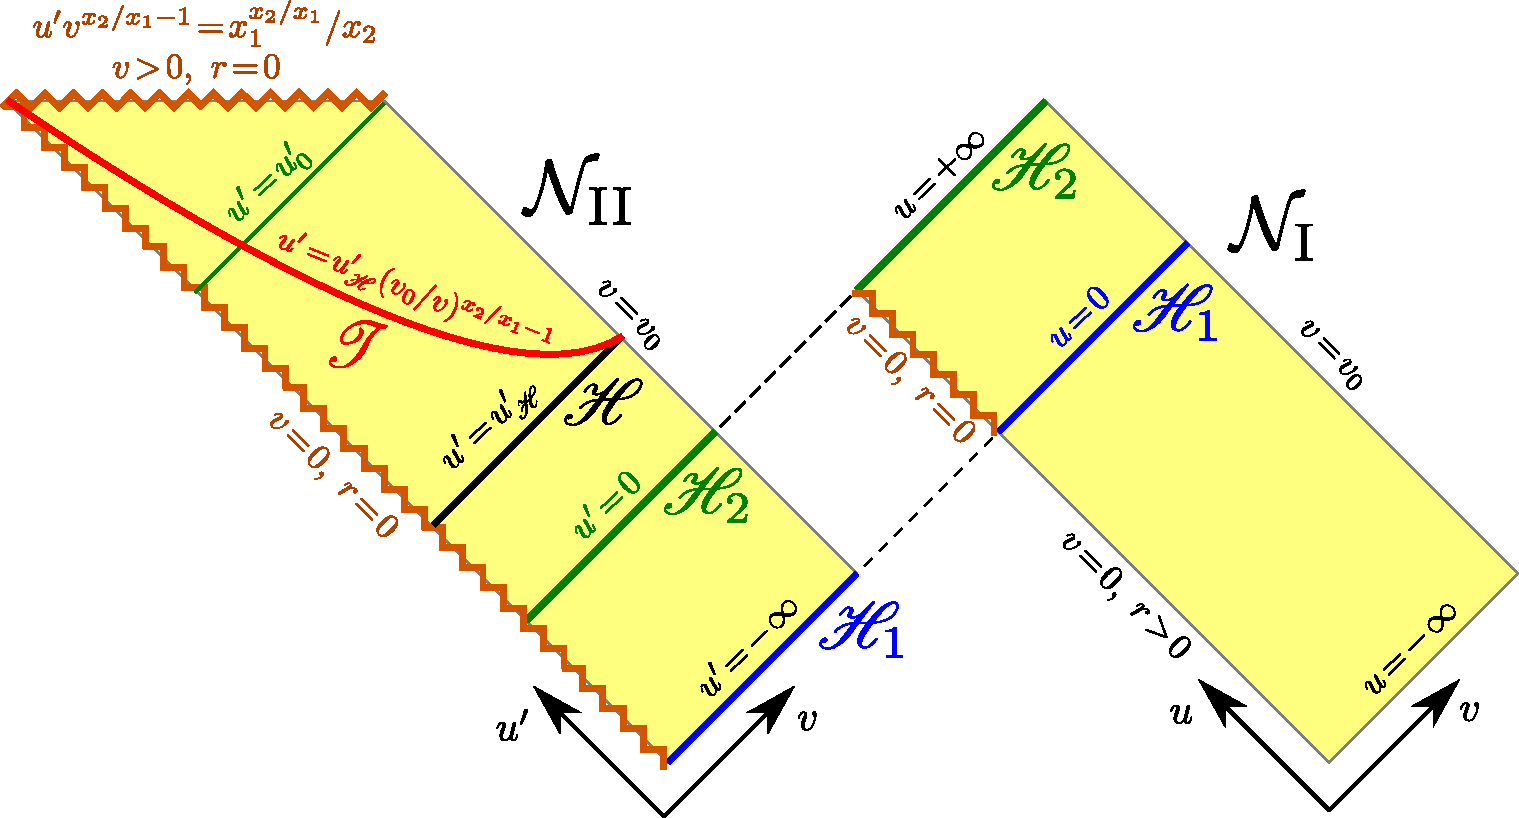
\includegraphics[width=0.8\textwidth]{vai_CPdiag_NI_NII.pdf}}
\caption[]{\label{f:vai:CPdiag_NI_NII} \footnotesize
Carter-Penrose diagrams of the subregions $\mathcal{N}_{\rm I}$ (right) and
$\mathcal{N}_{\rm II}$ (left) of the radiation region $\M_{\rm rad}$. The region
between the homothetic Killing horizons $\Hor_1$ and $\Hor_2$ is common to
both $\mathcal{N}_{\rm I}$ and $\mathcal{N}_{\rm II}$.
Zigzag lines indicate a curvature singularity. The red curve in $\mathcal{N}_{\rm II}$
is the trapping horizon $\mathscr{T}$ [Eq.~(\ref{e:vai:eq_T_NII})].
}
\end{figure}

\begin{example}
Let us perform a first order expansion in $v$ of the explicit expression of $r(u,v)$
found in Example~\ref{x:vai:u_r_1o9} [Eq.~(\ref{e:vai:r_uv_1o9})].
Taking into account the identity $\sqrt{u^2} = |u|$, we get
\be
\begin{cases}
 \displaystyle r = u^2 + \frac{1}{3} v + O(v^2) & \quad\mbox{for}\ u < 0 \\
 \displaystyle r = \frac{1}{6} v + O(v^2) & \quad\mbox{for}\ u > 0 .
\end{cases}
\ee
The first equation agrees with the relation $u = - r^{1 - x_1/x_2}$ found
above for $r \neq 0 $ and $v = 0$, given that $x_1/x_2 = 1/2$ in the present
case, while the
last equation is exactly (\ref{e:vai:r_v_0_N_I}), given that $x_2=6$.
\end{example}

As discussed above, the double null coordinates $(u, v, \th, \ph)$
are regular coordinates on $\mathscr{N}_{\rm I}$, because the components
(\ref{e:vai:metric_N_I}) of the metric tensor are regular (except for the
standard singularities of the spherical coordinates $(\th,\ph)$). Another advantage
of these coordinates is that they allow for an immediate drawing of
Carter-Penrose diagrams. It suffices to bring $u$ to a finite range by
setting e.g. $U = \arctan u$ and use the coordinates
$T = U + v$ and $X = v - U$ to get such a diagram of $\mathscr{N}_{\rm I}$,
as depicted in Fig.~\ref{f:vai:CPdiag_NI_NII}.

Let us describe the (vicinity of the) curvature singularity in the double null
coordinates. In the present case, where $M(v) = \alpha v/2$, the Kretschmann
scalar (\ref{e:vai:Kretschmann}) reduces to
\be \label{e:vai:Kretschmann:M_linear}
    K = 12\alpha^2 \frac{v^2}{r^6} ,
\ee
where $r$ is the function of $(u,v)$ given implicitly by Eq.~(\ref{e:vai:u_N_I})
(or explicitly by Eq.~(\ref{e:vai:r_uv_1o9}) in the case $\alpha=1/9$).
The above expression shows that
$K$ diverges only if $r\to 0$. This occurs only for $v \to 0$ in the
subregion $u\geq 0$ of $\mathscr{N}_{\rm I}$. There, Eq.~(\ref{e:vai:r_v_0_N_I})
leads to $K \sim 12 \alpha^2 x_2^6 / v^4$, which actually diverges as
$v \to 0$. We conclude that
\begin{greybox}
In $\mathscr{N}_{\rm I}$, the curvature
singularity corresponds to $u\geq 0$ and $v\to 0$.
\end{greybox}
This curvature singularity corresponds to the zigzag segment in
Fig.~\ref{f:vai:CPdiag_NI_NII} right.

\subsubsection{The $\mathscr{N}_{\rm II}$ region}

On $\mathscr{N}_{\rm II}$, let us introduce the parameter $u'$ to rewrite
$\tilde{c}$ in Eq.~(\ref{e:vai:v_r_out_naked}) as
\be \label{e:vai:def_up_tilde_c}
    \tilde{c} = |u'|^{x_1/(x_2 - x_1)} .
\ee
Then Eq.~(\ref{e:vai:v_r_out_naked}) yields $|u'| = |v/x_2 - r| / (v/x_1 - r)^{x_2/x_1}$.
Choosing the sign of $u'$ such that $u'\to -\infty$ at the outer boundary of
$\mathscr{N}_{\rm II}$ ($r\to v/x_1$), we get
\be \label{e:vai:up_N_II}
    \encadre{ u' = \frac{v/x_2 - r}{\left(v/x_1 - r \right)^{x_2/x_1}} }.
\ee
We may then consider $(u',v,\th,\ph)$ as a coordinate system on $\mathscr{N}_{\rm II}$.
\begin{remark}
Contrary to the range of $u$ on $\mathscr{N}_{\rm I}$, which is $(-\infty,+\infty)$,
the range of $u'$ on $\mathscr{N}_{\rm II}$ is bounded from above by a function
of $v$, which is given by Eq.~(\ref{e:vai:range_v_uprime}) below.
\end{remark}
As above, the metric components in coordinates $(u',v,\th,\ph)$
are deduced from those in coordinates $(v,r,\th,\ph)$ [Eq.~(\ref{e:vai:self_similar_metric})]
(cf. the notebook~\ref{s:sam:Vaidya_nk_sing} for the computation):
\be
    \w{g} = - \frac{2 x_1}{(x_2 - x_1)r} \left(\frac{v}{x_1} - r \right)^{x_2/2}
        \dd u' \, \dd v
        + r^2 \left( \dd\th^2 + \sin^2\th\, \dd\ph^2 \right) \qquad
        \left( r < \frac{v}{x_1}\right) ,
\ee
where $r = r(u', v)$ is defined implicitly by Eq.~(\ref{e:vai:up_N_II}).
Again, we get a double-null coordinate system adapted to the ingoing and
outgoing radial null geodesics. Moreover, the coordinates $(u',v,\th,\ph)$ are regular
since $g_{u'v}$ is finite and non-vanishing in all $\mathscr{N}_{\rm II}$.
In addition, the homothetic Killing horizon $\Hor_2$,
which is defined by $v/r = x_2$, is the hypersurface $u' = 0$ of $\mathscr{N}_{\rm II}$.
In $\mathscr{N}_{\rm I}\cap \mathscr{N}_{\rm II}$, we have $u>0$ and $u'<0$.
The relation between the two coordinates is obtained by equating the
right-hand sides of Eqs.~(\ref{e:vai:def_u_tilde_c}) and (\ref{e:vai:def_up_tilde_c});
one gets
\be \label{e:vai:up_u}
    u' = - u^{-x_2/x_1} \quad\mbox{in}\ \mathscr{N}_{\rm I}\cap \mathscr{N}_{\rm II} ,
\ee
along with the following characterization of the two homothetic Killing horizons
(cf. Fig.~\ref{f:vai:CPdiag_NI_NII}):
\begin{subequations}
\begin{align}
\Hor_1:\quad &u = 0, \quad u' \to - \infty \\
\Hor_2:\quad &u \to +\infty, \quad u'=0 .
\end{align}
\end{subequations}

\begin{example}
For $\alpha=1/9$, i.e. $x_1 = 3$ and $x_2 = 6$,
Eq.~(\ref{e:vai:up_N_II}) reduces to
\be \label{e:vai:up_v_r_alp1o9}
    u' = \frac{3}{2} \frac{v - 6r}{(v - 3 r)^2} .
\ee
This relation can be inverted, yielding  an explicit expression for $r(u', v)$:
\be \label{e:vai:r_up_v_alp1o9}
    r = \frac{v}{3} + \frac{1}{2u'} \left( \sqrt{1 - \frac{2}{3} u' v } - 1 \right) .
\ee
Equation~(\ref{e:vai:up_u}) reduces to
\be
    u' = - \frac{1}{u^2} \quad\mbox{in}\ \mathscr{N}_{\rm I}\cap \mathscr{N}_{\rm II} .
\ee
Substituting this expression for $u'$ in Eq.~(\ref{e:vai:r_up_v_alp1o9}), one recovers
Eq.~(\ref{e:vai:r_uv_1o9}).
\end{example}

Let us locate the curvature singularity at the boundary of $\mathscr{N}_{\rm II}$.
A necessary condition for the Kretschmann scalar (\ref{e:vai:Kretschmann:M_linear})
to diverge is $r(u',v) \to 0$. According to Eq.~(\ref{e:vai:r_to_0_outgoing}),
this occurs along an outgoing radial null
geodesic if, and only if, $x \to x_2$ or $x\to +\infty$.
Now, let us rewrite Eq.~(\ref{e:vai:up_N_II}) by substituting $x r$ for $v$:
\[
    u' = \frac{x/x_2 - 1}{\left(x/x_1 - 1 \right)^{x_2/x_1} r^{x_2/x_1-1}} .
\]
Since $u'$ is fixed along the outgoing radial null geodesic, we recover
from this expression the two limits $x \to x_2$ or $x\to +\infty$ in which
$r(u',v) \to 0$ may occur. The first limit corresponds to $v \sim x_2 r$
(actually the same behavior as (\ref{e:vai:r_v_0_N_I}) in $\mathscr{N}_{\rm I}$),
which implies $v\to 0$. This leads to
$K \sim 12\alpha^2 x_2^6/v^4$, which does diverge for $v\to 0$.
For the second limit, $x \to +\infty$, we get
\[
    u' \sim \frac{x_1^{x_2/x_1}}{x_2 (x r)^{x_2/x_1 - 1}} .
\]
This implies that $x r = v$ tends to a finite value. Then $K = 12\alpha^2 v^2 / r^6$
diverges as $r^{-6}$ there. In conclusion:
\begin{greybox}
In $\mathscr{N}_{\rm II}$,
the limit $r\to 0$ corresponds to a curvature singularity.
This singularity is reached in two places, which constitute parts of the boundary
of $\mathscr{N}_{\rm II}$: (i) $v\to 0$ (the zigzag segment inclined
at $45^\circ$ in Fig.~\ref{f:vai:CPdiag_NI_NII} left) and (ii) $u' v^{x_2/x_1 - 1}
\to x_1^{x_2/x_1} / x_2$ (the horizontal zigzag segment in Fig.~\ref{f:vai:CPdiag_NI_NII} left). In particular, the ranges of the coordinates
$(u',v)$ in $\mathscr{N}_{\rm II}$ are
\be \label{e:vai:range_v_uprime}
    0 < v \leq v_0 \qand
    -\infty < u' < \frac{x_1^{x_2/x_1}}{x_2 v^{x_2/x_1 - 1}} .
\ee
\end{greybox}

\begin{example}
For $\alpha=1/9$, i.e. $x_1 = 3$ and $x_2 = 6$,
Eq.~(\ref{e:vai:r_up_v_alp1o9}) implies
\be
\lim_{v\to 0} r = 0 \qand
\lim_{u'v\to 3/2} r = 0 .
\ee
The second limit agrees with the upper boundary for $u'$
in (\ref{e:vai:range_v_uprime}), since the latter can be
rewritten as $u'  < 3/(2 v)$
for $x_1 = 3$ and $x_2 = 6$.
\end{example}


As a particular case of Eq.~(\ref{e:vai:range_v_uprime}), the maximal
value of $u'$ along an ingoing radial null
geodesic with $v = v_0$ (geodesic on the outer edge of the radiation shell,
cf. Fig.~\ref{f:vai:CPdiag_NI_NII})
is
\be \label{e:vai:nak:up0}
    u'_0 = \frac{x_1^{x_2/x_1}}{x_2 v_0^{x_2/x_1 - 1}} .
\ee

\begin{figure}
\centerline{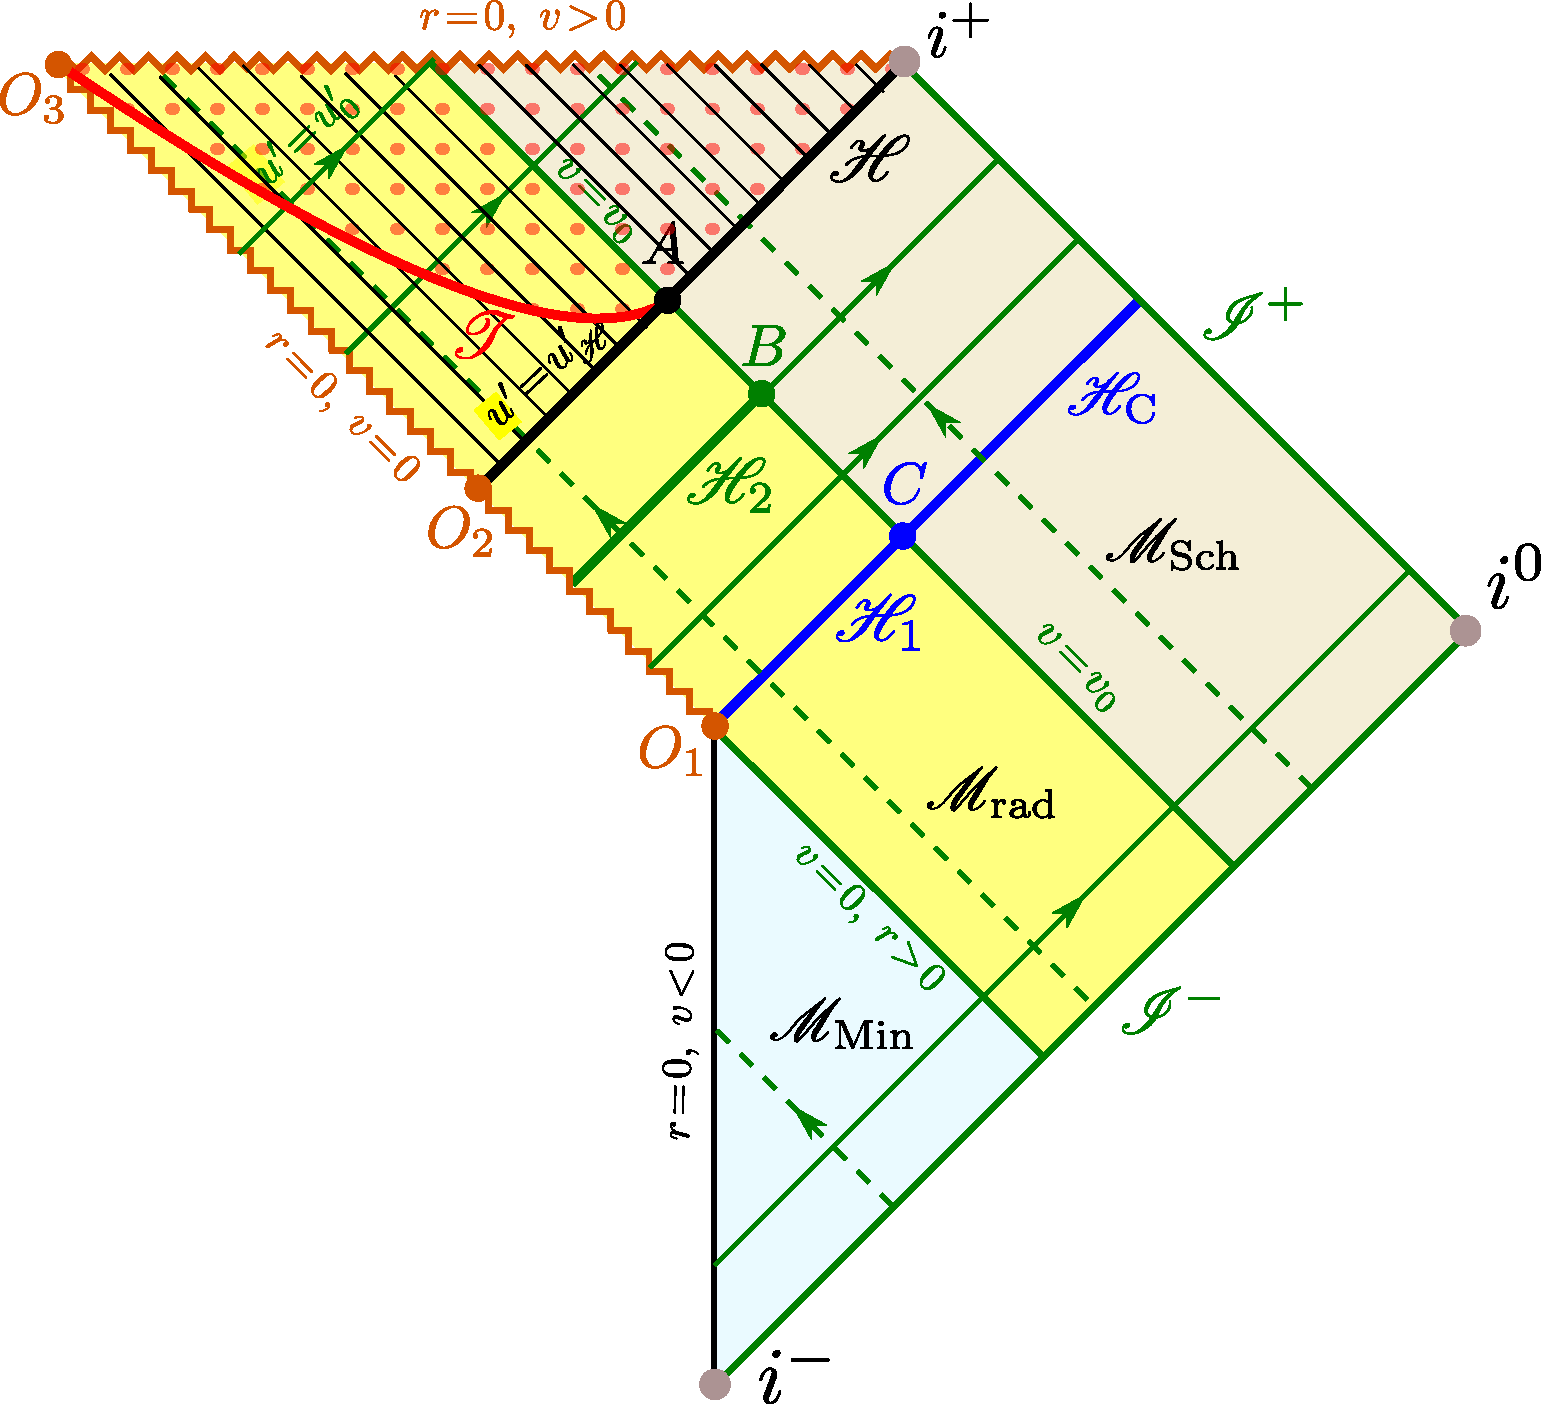
\includegraphics[width=0.7\textwidth]{vai_CPdiag_nk_sing.pdf}}
\caption[]{\label{f:vai:CPdiag_nk_sing} \footnotesize
Carter-Penrose diagram of the collapsing Vaidya spacetime with
$M(v) = \alpha v /2$ (homothetic radiation region)
and $\alpha < 1/8$ (low energy density case).
The Minkowski region $\M_{\rm Min}$, radiation region $\M_{\rm rad}$
and Schwarzschild region $\M_{\rm Sch}$ are depicted in respectively
pale blue, yellow and grey.
Solid (resp. dashed) green lines are outgoing (resp. ingoing)
radial null geodesics.
Zigzag lines indicate curvature singularities.
The hatched area is the black hole region,
delimited by the event horizon $\Hor$.
The red dot-filled area, delimited by the future outer trapping horizon
$\mathscr{T}$ (red curve),
is the region where the spheres $(t,r)=\mathrm{const}$
are trapped surfaces.
The points $A$, $B$ and $C$
are the same as in Fig.~\ref{f:vai:diag_naked_S0}, while the point $O$
of Fig.~\ref{f:vai:diag_naked_S0} corresponds to the whole segment
$O_1 O_3$.
}
\end{figure}

\subsection{Carter-Penrose diagram of the whole spacetime}

A Carter-Penrose diagram of the whole Vaidya spacetime can be constructed
by assembling the Carter-Penrose diagrams obtained for the radiation region
$\M_{\rm rad}$ (Fig.~\ref{f:vai:CPdiag_NI_NII}) with Carter-Penrose diagrams of the Minkowski
region ($v<0$) and of the Schwarzschild region ($v> v_0$).
To achieve this, one should locate the black hole event horizon $\Hor$
in $\M_{\rm rad}$.
Given that $x_A = \alpha^{-1} >  x_1$ (cf. Sec.~\ref{s:vai:low_alpha}),
one has $\Hor\cap \M_{\rm rad} \subset
\mathcal{N}_{\rm II}$.
Since $\Hor$ is generated by outgoing radial
null geodesics, $\Hor\cap \M_{\rm rad}$ lies a constant value of $u'$, which
we shall denote by $u'_\Hor$. The value of ${u'}_\Hor$ is obtained by
setting $v=v_0$ and $r=2m$ in Eq.~(\ref{e:vai:up_N_II}). Using the identities
$\alpha = 2m/v_0$ and $\alpha = 2/(x_1 x_2)$, we get
\be \label{e:vai:nak:upH}
    u'_\Hor = u'_0 \left(1 - \frac{2}{x_1} \right)
    \left(1 - \frac{2}{x_2} \right)^{-x_2/x_1} .
\ee
From the expressions of $x_1$ and $x_2$ in terms of $\alpha$
[Eq.~(\ref{e:vai:x1_x2})], it is easy to show that $u'_\Hor < u'_0$.
Taking this property into account, one can draw $\Hor$ in the diagram of $\mathscr{N}_{\rm II}$
of Fig.~\ref{f:vai:CPdiag_NI_NII} and finally obtain
the Carter-Penrose diagram of $\M$ shown in
Fig.~\ref{f:vai:CPdiag_nk_sing}.

\begin{example}
For $v_0 = 18 m$, one has $\alpha = 1/9$, $x_1 = 3$ and $x_2 = 6$, so that Eqs.~(\ref{e:vai:nak:up0})
and (\ref{e:vai:eq_T_NII}) yield respectively
$u'_0 = 3/(2 v_0) = 1/(12 m)$ and
$u'_\Hor = 3 u'_0 / 4=  9/(8 v_0) = 1/(16 m)$.
\end{example}

The Carter-Penrose diagram of Fig.~\ref{f:vai:CPdiag_nk_sing} enables us to fully solve the puzzle of multiple outgoing radial null geodesics emanating from the point $(t,r) = (0,0)$ raised at the beginning of
Sec.~\ref{s:vai:analysis_double_null}: $(t,r) = (0,0)$, or equivalently, $(v, r) = (0,0)$,
does not define a single point, but a full segment, denoted by $O_1 O_3$ in Fig.~\ref{f:vai:CPdiag_nk_sing}. From each point of this segment, there emanates a single outgoing radial null geodesic (cf. the green solid lines in Fig.~\ref{f:vai:CPdiag_nk_sing}).

It is instructive to add the future outer trapping horizon $\mathscr{T}$
introduced in Sec.~\ref{s:vai:trapped_surf}
to the Carter-Penrose diagram. To do so, we need the equation of $\mathscr{T}$
in terms of the double null coordinates. First of all, we notice that in $\M_{\rm rad}$, $\mathscr{T}$ is
entirely contained in $\mathscr{N}_{\rm II}$. Indeed, $\mathscr{T}$ obeying
$r = \alpha v$ [Eq.~(\ref{e:vai:def_T_hom})], the property $\alpha < x_2^{-1}$
excludes $\mathscr{T}$ from $\mathscr{N}_{\rm I}$, by the definition
(\ref{e:vai:def_NI_NII}) of the latter. It suffices then to express  $\mathscr{T}$ in terms of the coordinates $(u',v)$ of  $\mathscr{N}_{\rm II}$.
This is acheived by substituting $\alpha v$ for $r$ in Eq.~(\ref{e:vai:up_N_II}) and making use of successively the identity $\alpha = 2/(x_1 x_2)$,
Eq.~(\ref{e:vai:nak:upH}) and Eq.~(\ref{e:vai:nak:up0}); one gets
\be \label{e:vai:eq_T_NII}
    \mathscr{T} \cap \M_{\rm rad}:\qquad
    u' = u'_\Hor \left(\frac{v_0}{v}\right) ^{x_2/x_1 - 1} .
\ee
Note that this implies $u'\to +\infty$ for $v\to 0$ and
$u'\to u'_\Hor$ for $v\to v_0$ (cf. Fig.~\ref{f:vai:CPdiag_NI_NII}).
\begin{example}
For our favorite example $\alpha = 1/9$ ($x_1 = 3$ and $x_2 = 6$),
the equation of $\mathscr{T} \cap \M_{\rm rad}$ reduces
to $u' = u'_\Hor v_0/v$, which corresponds to a branch of hyperbola in the $(u',v)$ plane.
\end{example}

\begin{hist}
The split of $\M_{\rm rad}$ in two regions, denoted here $\mathscr{N}_{\rm I}$
and $\mathscr{N}_{\rm II}$, in order to get regular double-null coordinate
systems, has been performed by
B. Waugh\index{Waugh, B.} and Kayll Lake\index{Lake, K.} in 1986 \cite{WaughL86}.
The double-null coordinates $(u,v)$ and $(u',v)$ introduced above are
theirs, except for some constant factors.
Four years before, William A. Hiscock\index{Hiscock, W.A.}, Leslie G. Williams\index{Williams, L.G.} and Douglas M. Eardley\index{Eardley, D.M.} \cite{HiscoWE82}
exhibited a Carter-Penrose diagram similar to that Fig.~\ref{f:vai:CPdiag_nk_sing}
except that it regards a case for which
the Cauchy and event horizons coincide (Fig.~2 in Ref.~\cite{HiscoWE82}),
which is obtained by adding a surface layer (Dirac delta) of radiation at $v=v_0$.
However, as discussed in Ref.~\cite{WaughL86}, these authors have not set up
regular double-null coordinates in $\M_{\rm rad}$, so that their construction
can be seen as rather heuristic. In 1984, Yuhji Kuroda\index{Kuroda, Y.} \cite{Kurod84}
exhibited a Carter-Penrose diagram again similar to that of Fig.~\ref{f:vai:CPdiag_thin}, except
for the radiation region extending to $\scri^+$ (no pure Schwarzschild exterior but
$M'(v) \to 0$ for $v\to +\infty$) (Fig. 3 in Ref.~\cite{Kurod84}). The case of a
radiation region bounded by $v = v_0$, as here, can be found in Fig.~1 of a 2007 article by
Brien C. Nolan\index{Nolan, B.C} \cite{Nolan07}.
\end{hist}


\subsection{Naked singularity and Cauchy horizon} \label{s:vai:nak_Cauchy}

We recover on the Carter-Penrose diagram of Fig.~\ref{f:vai:CPdiag_nk_sing}
the naked singularity\index{naked singularity}\index{singularity!naked --} feature noticed in Sec.~\ref{s:vai:low_alpha}:
it appears clearly
that light rays emitted by the curvature singularity
between $O_1$ and $O_2$ can reach the future null infinity $\scri^+$ of the
Schwarzschild exterior. This means that the singularity is visible to
remote observers (cf. observer $\Obs$ in Fig.~\ref{f:vai:CPdiag_Cauchy}).
This contrasts with the curvature singularity of the
Vaidya collapse with $v_0 < 16 m$ (compare Fig.~\ref{f:vai:CPdiag_thin}
with Fig.~\ref{f:vai:CPdiag_nk_sing}).
The latter is indeed located at the ``future boundary'' of spacetime, so that
no causal geodesic can originate from it.

\begin{figure}
\centerline{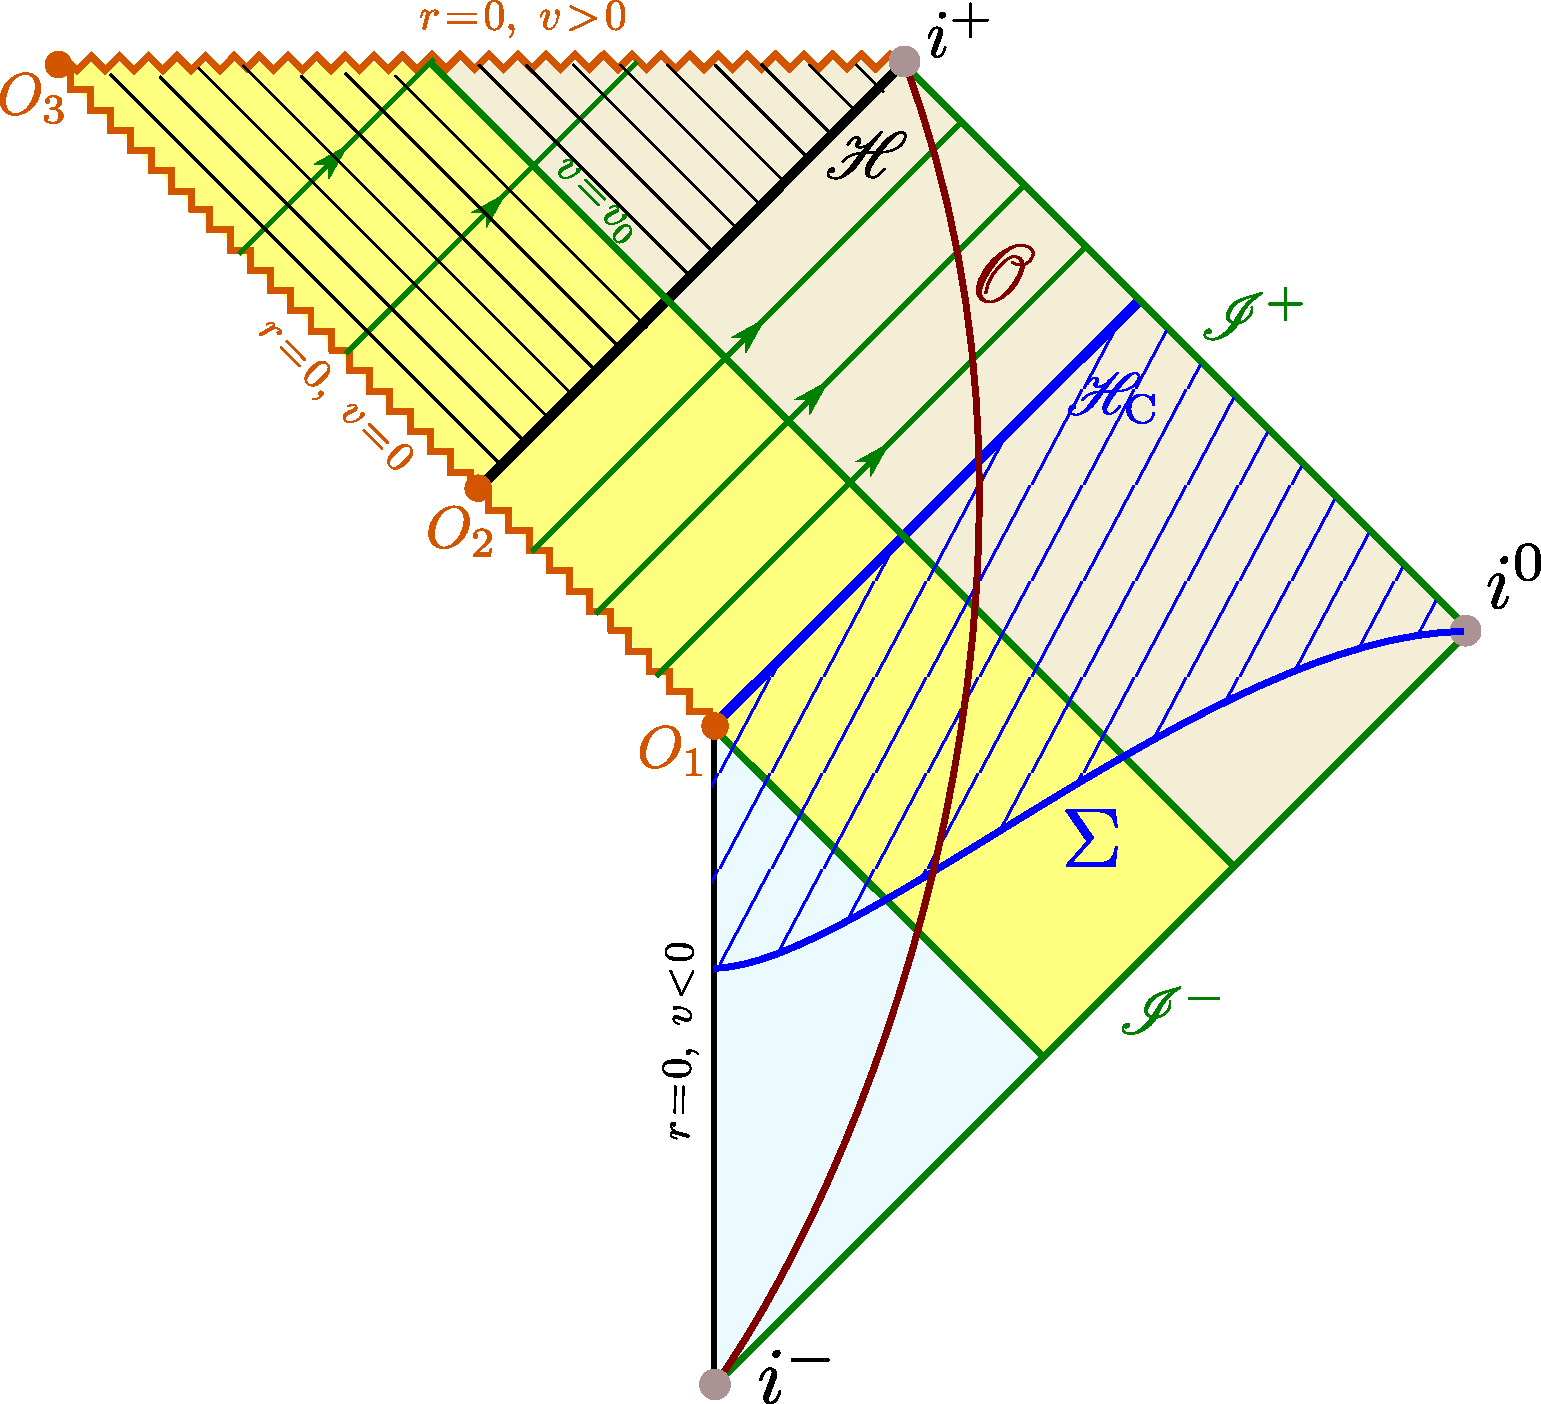
\includegraphics[width=0.7\textwidth]{vai_CPdiag_Cauchy.pdf}}
\caption[]{\label{f:vai:CPdiag_Cauchy} \footnotesize
Same as Fig.~\ref{f:vai:CPdiag_nk_sing}, with in addition the remote
observer $\Obs$, the partial Cauchy surface $\Sigma$ and its future Cauchy development $D^+(\Sigma)$ (blue hatched area, cf. Sec.~\ref{s:ker:Cauchy_hor} for the definition), which is bounded in the future by
the Cauchy horizon $\Hor_{\rm C}$ and the future null infinity $\scri^+$.}
\end{figure}

\begin{remark}
The part $O_2 O_3$ of the curvature singularity (cf. Fig.~\ref{f:vai:CPdiag_nk_sing})
is visible to observers that fall into the black hole, but remains hidden
to remote observers. For this reason, the singularity $O_2 O_3$ is qualified as
\defin{locally naked}\index{naked singularity!locally --}\index{singularity!locally naked --},
while $O_1 O_2$ is qualified as
\defin{globally naked}\index{naked singularity!globally --}\index{singularity!globally naked --}.
For remote observers, one may say that the
singularity $O_2 O_3$ is ``clothed'' by the event horizon $\Hor$.
\end{remark}

\begin{remark}
The curvature singularity of the Vaidya spacetime with $v_0 < 16 m$ (Fig.~\ref{f:vai:CPdiag_thin})
is not even locally naked: observers falling into the black hole region never see
it until they hit it at the end of their lives.
\end{remark}

The part  $(v, r) = (0, 0)$ of the curvature singularity, i.e. the segment $O_1 O_3$ in
the diagram of Fig.~\ref{f:vai:CPdiag_nk_sing} corresponds to a past null boundary of
spacetime.
Such a singularity is generically called a
\defin{shell-focusing singularity}\index{shell-focusing singulariy}\index{singularity!shell-focusing --}. This terms has been coined by Eardley \& Smarr \cite{EardlS79}, who discovered them
in spherically symmetric inhomogeneous dust collapse.
Due to its past null character, a shell-focusing singularity is always locally naked: close observers can see it.



Remote observers see the naked singularity as soon as they cross
the null hypersurface $\Hor_{\rm C}$ generated by the outgoing radial null geodesics
emanating from the birth of the singularity at $u=0$ in $\mathscr{N}_{\rm I}$
(point $O_1$ in Figs.~\ref{f:vai:CPdiag_nk_sing} and \ref{f:vai:CPdiag_Cauchy} ).
$\Hor_{\rm C}$ can be seen as the null hypersurface extending the
homothetic Killing horizon $\Hor_1$ beyond the radiation region, i.e. one has
$\Hor_{\rm C} \cap \M_{\rm rad} = \Hor_1$.
The hypersurface $\Hor_{\rm C}$ is actually the future Cauchy horizon\index{future!Cauchy!horizon}\index{Cauchy!horizon}\index{horizon!Cauchy --} (cf. Sec.~\ref{s:ker:Cauchy_hor})
of any partial Cauchy surface $\Sigma$ that encounters the Minkowkski region\footnote{Since it
has to be acausal without edge (cf. Sec.~\ref{s:ker:Cauchy_hor}), $\Sigma$ has to meet the spacelike infinity $i^0$
in the Carter-Penrose diagram of Fig.~\ref{f:vai:CPdiag_Cauchy} (cf. Fig.~\ref{f:vai:CPdiag_Cauchy})}.
In other words, the region of spacetime in the future of $\Hor_{\rm C}$ cannot
be entirely predicted from initial data on $\Sigma$ and the Einstein equations.
In particular, data from the naked curvature singularity $O_1 O_3$ is required.
Since a curvature singularity marks a validity limit of general relativity,
one cannot unambiguously prescribe data there. This seriously hampers the
predictability of general relativity alone for describing the region
beyond $\Hor_{\rm C}$. For instance, a huge burst of radiation could come
out at any time from the naked singularity and change the fate of observers
travelling in this region. In particular, this regards all remote observers at a sufficiently
advanced amount of their proper time, since any such observer necessarily crosses
$\Hor_{\rm C}$ at some point (cf. observer $\Obs$ in Fig.~\ref{f:vai:CPdiag_Cauchy},
noticing that the worldlines of all remote observers
terminate at the future timelike infinity $i^+$).



%%%%%%%%%%%%%%%%%%%%%%%%%%%%%%%%%%%%%%%%%%%%%%%%%%%%%%%%%%%%%%%%%%%%%%%%%%%%%%%


\section{Going further}

For simplicity, we have mostly restricted ourselves to $M(v)$ linear in the radiation
region, except in Secs.~\ref{s:vai:thin:sing} and \ref{s:vai:trapped_surf}.
This allowed us to benefit from an extra symmetry (homothetic Killing vector) and to get
exact solutions for the outgoing radial null geodesics.
The obtained results are nevertheless representative of those for more
general functions
$M(v)$. In particular, the criterion for having a shell-focusing singularity\index{shell-focusing singularity}\index{singularity!shell-focusing --}
with a generic function $M(v)$ remains $\alpha < 1/8$ but with $\alpha$ defined
by
\be
    \alpha := \lim_{v\to 0^+} \frac{2 M(v)}{v} .
\ee
See Ref.~\cite{Kurod84,FayosT08} for details. Of course, for $M(v) = m v /v_0$, the
above definition of $\alpha$ reduces to (\ref{e:vai:def_alpha}).
For $\alpha < 1/8$, a new possibility may occur: that of a shell-focusing singularity
that lies entirely in the black hole region, i.e. that is naked locally but not globally,
contrary to what happens for $M(v)$ linear (Sec.~\ref{s:vai:naked_sing}).
See e.g. Fig.~4 of Ref.~\cite{AshteK04} or Fig.~9.20 of Ref.~\cite{GriffP09}
for the corresponding Carter-Penrose diagram.
Actually, the Vaidya collapse depicted in Fig.~\ref{f:vai:diag_S2} lies in this
category: it has $M(v) = m (v/v_0)^3 \left[ 6 (v/v_0)^2 - 15 v/v_0 + 10 \right]$,
so that $\alpha = 0$. The singularity is entirely located in the black
hole region and appears to be locally naked (note the outgoing radial null geodesic
emerging from it near $(t,r) = (0,0)$ in Fig.~\ref{f:vai:diag_S2}).

It is worth to stress that in the literature,
many studies regard the \emph{outgoing} Vaidya metric, starting from the original studies
(cf. the historical note on p.~\pageref{h:vai:origin}), because they are
motivated either by the modelling of radiating bodies or the
study of black hole evaporation. Nonetheless, most results are applicable
to Vaidya collapse (which is based on the
\emph{ingoing} version of the metric) by performing some time reversal.
For instance, one can infer from the recent study \cite{CoudrN21}
that for an imploding Vaidya spacetime without any Minkowksi region
($v$ spanning the range $(-\infty, v_0)$ in the radiation region),
but such that $\lim_{v\to -\infty} M(v) = 0$, there is a curvature singularity
at the null boundary $v\to -\infty$ of spacetime, whatever the choice of the
non-decreasing mass function $M(v)$.
%\cite{Krish14}



